\documentclass[xcolor=table]{beamer}
\usepackage[utf8]{inputenc}
\usepackage{listings}
\usepackage{adjustbox}
\usepackage{graphicx}
\usepackage{wrapfig}
\usepackage{tikz}  
\usepackage[norsk]{babel}
\usepackage{caption}
\captionsetup{font=scriptsize,labelfont=scriptsize}

\usepackage[
    backend=biber,
    style=numeric,
    sorting=none
]{biblatex}
\addbibresource{thesis/refs.bib}

\title[Spoof proof GPS timing] % (optional, only for long titles)
{Spoof proof GPS timing}
\subtitle{A detection and mitigation system for GPS time spoofing}
\author[A. Schultzen] % (optional, for multiple authors)
{A.~Schultzen\inst{1}}
\institute[Universities Here and There] % (optional)
{
  \inst{1}%
  Institutt for informatikk\\
  Universitetet i Oslo
}

\setcounter{tocdepth}{1}
\date{\today}
\usetheme{Marburg}

\begin{document}

\frame{\titlepage}

\section{Introduksjon}
  \frametitle{Introduksjon}
\begin{frame}
  Laget et rammeverk for å teste forskjellige spoofing deteksjonsalgoritmer. Ikke gjort før.
\end{frame}

\subsection{GPS timing}
\begin{frame}
\frametitle{GPS timing} 
  \begin{figure}
  \vspace{-30pt}
      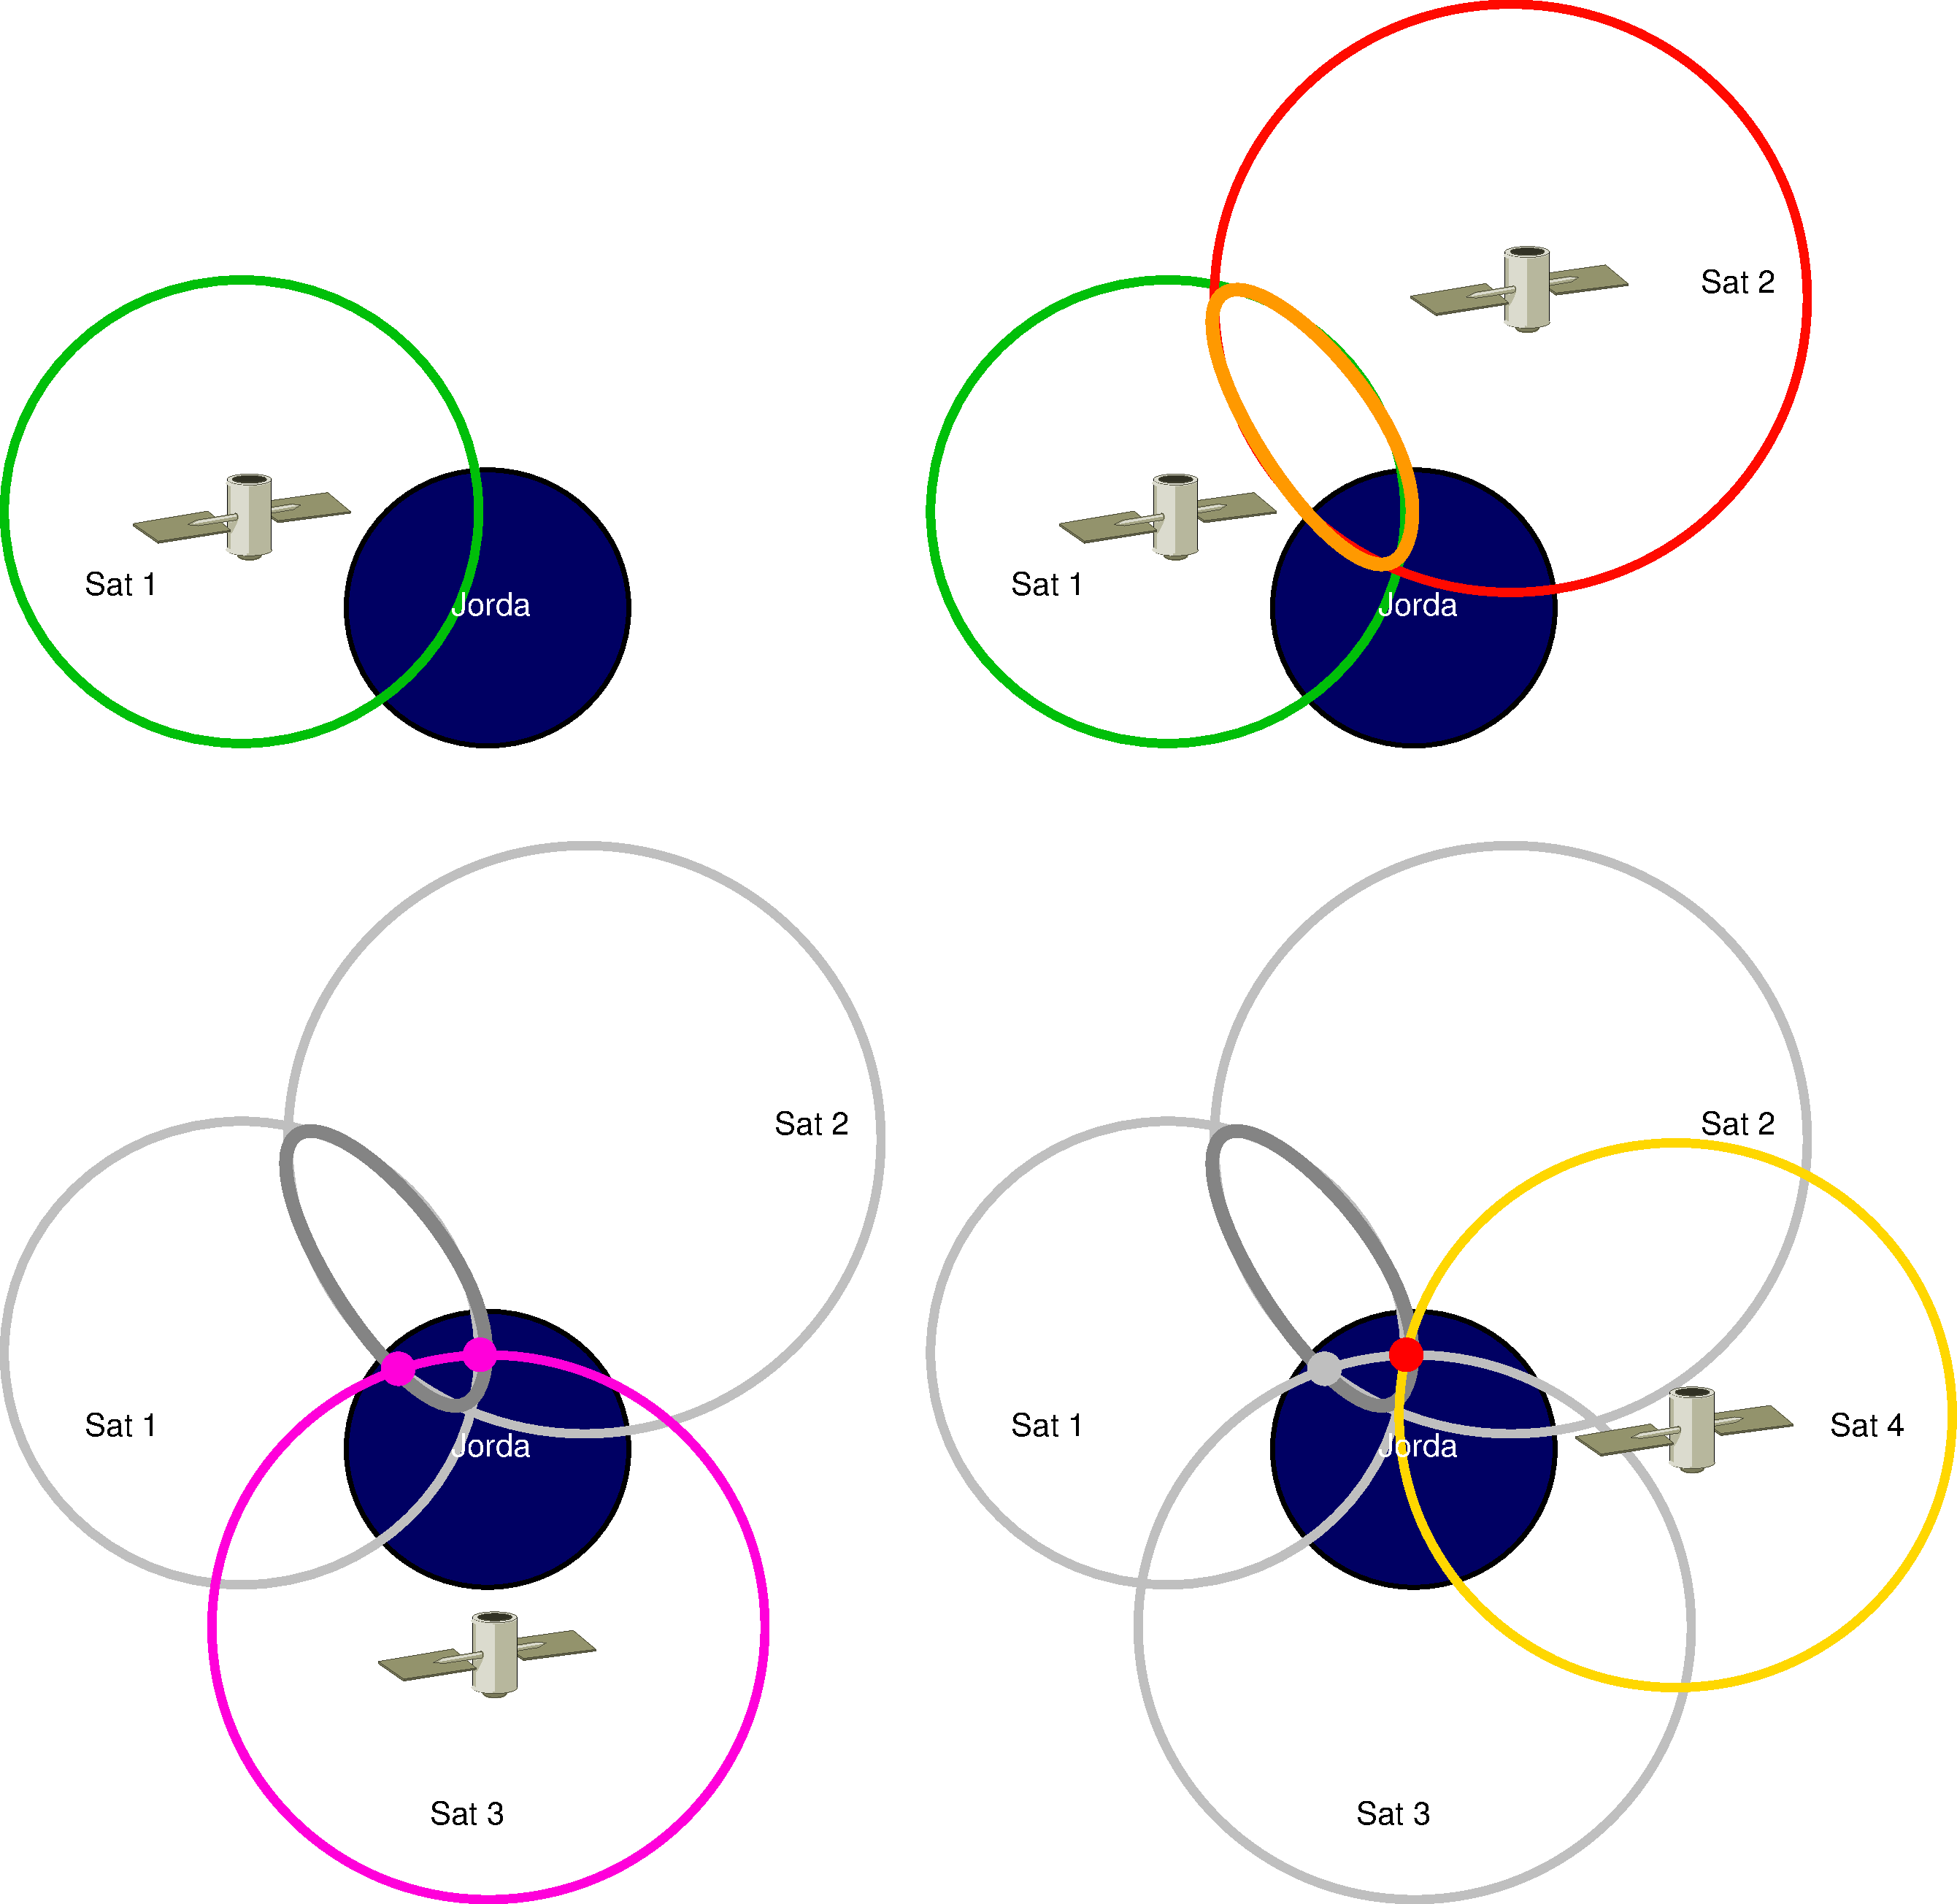
\includegraphics[scale=0.17]{thesis/graphics/trilaterate.pdf}
      \caption{Trilaterasjon}
    \end{figure}
\end{frame}

\subsection{Anvendelse}
\begin{frame}
\frametitle{GPS timing}
  \begin{columns}
    \column{0.3\textwidth}
          \hspace{-50pt}
      \begin{figure}
        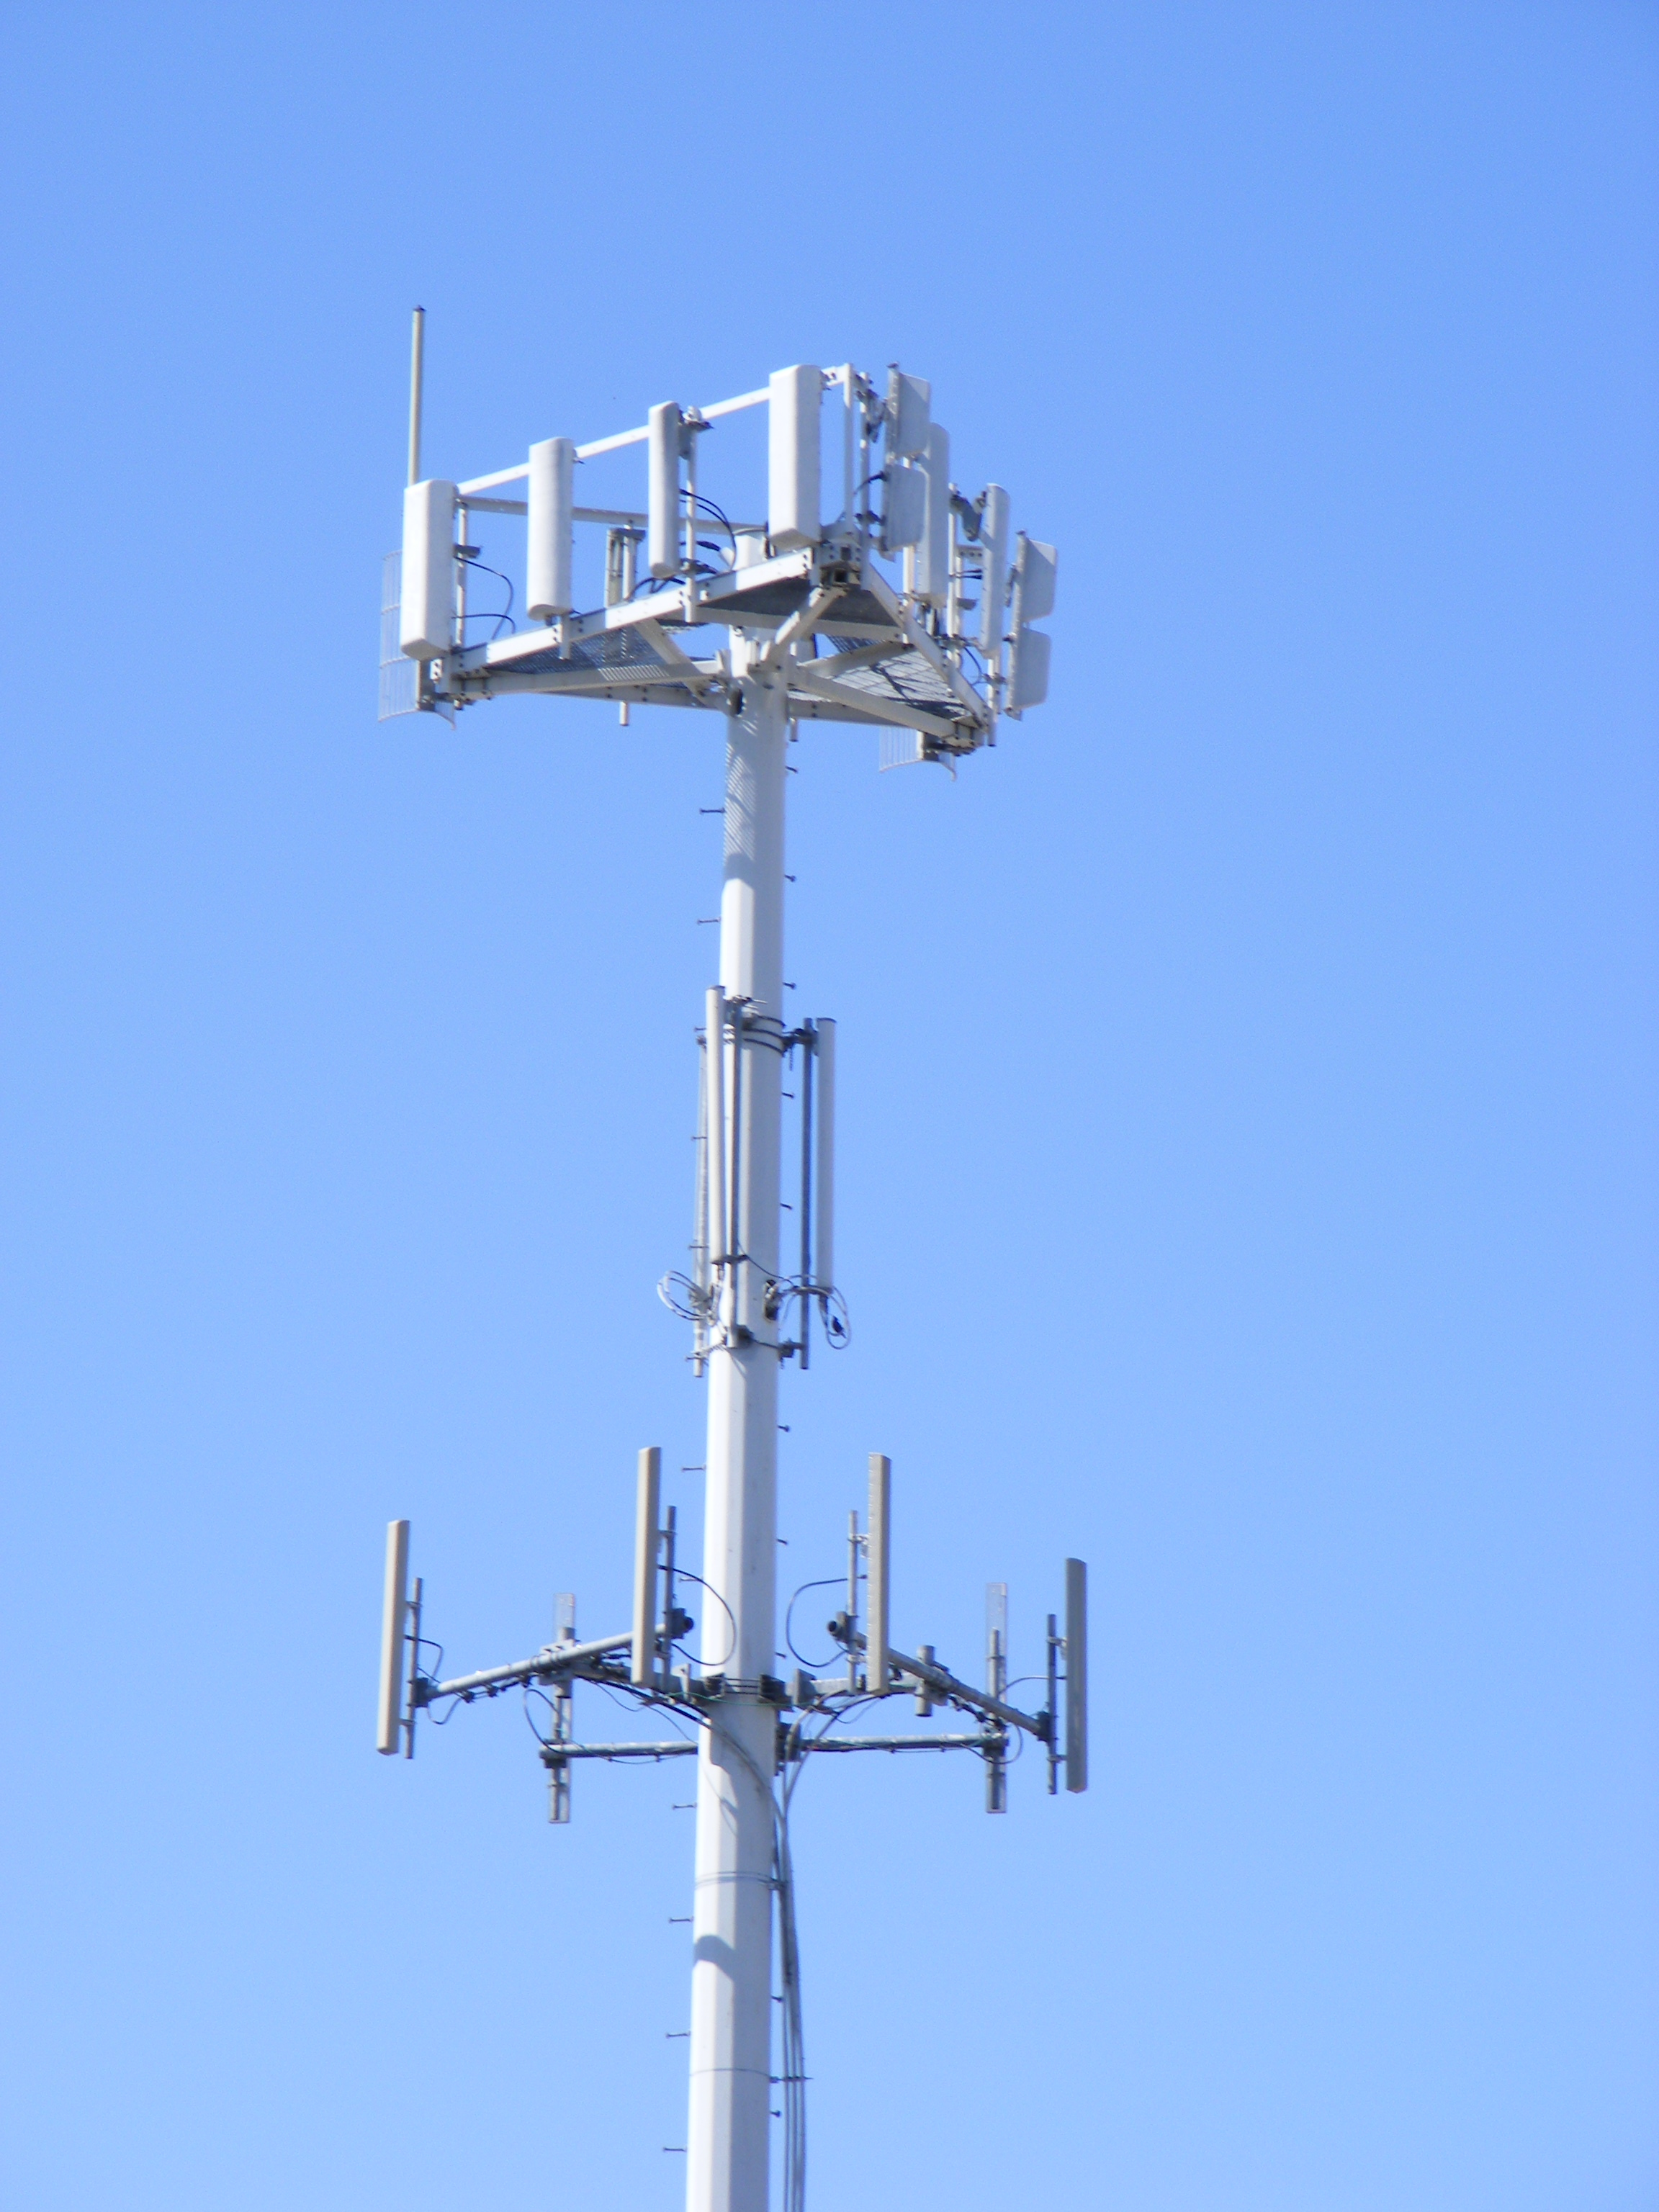
\includegraphics[scale=0.045]{thesis/graphics/Cell-Tower.jpg}
        \caption{Mobilmast \cite{CELLTOWER}}
      \end{figure}

    \column{0.3\textwidth}
              \hspace{-50pt}
      \begin{figure}
        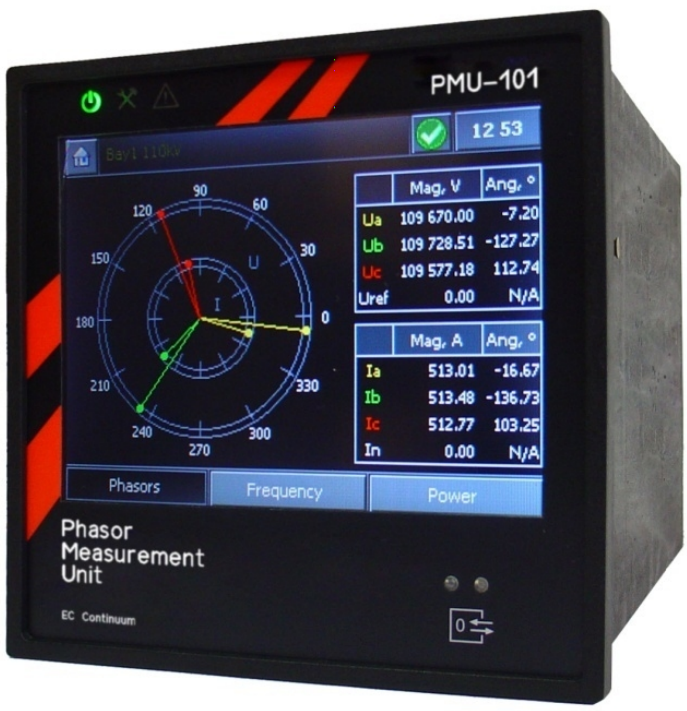
\includegraphics[scale=0.1]{thesis/graphics/pmu.png}
        \caption{PMU \cite{PMU}}
      \end{figure}
    %\begin{itemize}
    %    \item Tidsstempling 
    %    \item Fasemålinger i kraftnett.
    %    \item Telekommunikasjon.
    %\end{itemize}
    \column{0.3\textwidth}
              \hspace{-100pt}
    \begin{figure}
        \includegraphics[scale=0.025]{thesis/graphics/New_York_Stock_Exchange,_Wall_Street.jpg}
        \caption{Wall Street \cite{NEWYORK}}
      \end{figure}
  \end{columns}
\end{frame}

\subsection{Utfordringer og trusler}
\begin{frame}
\frametitle{Utfordringer og trusler}
      \begin{figure}
        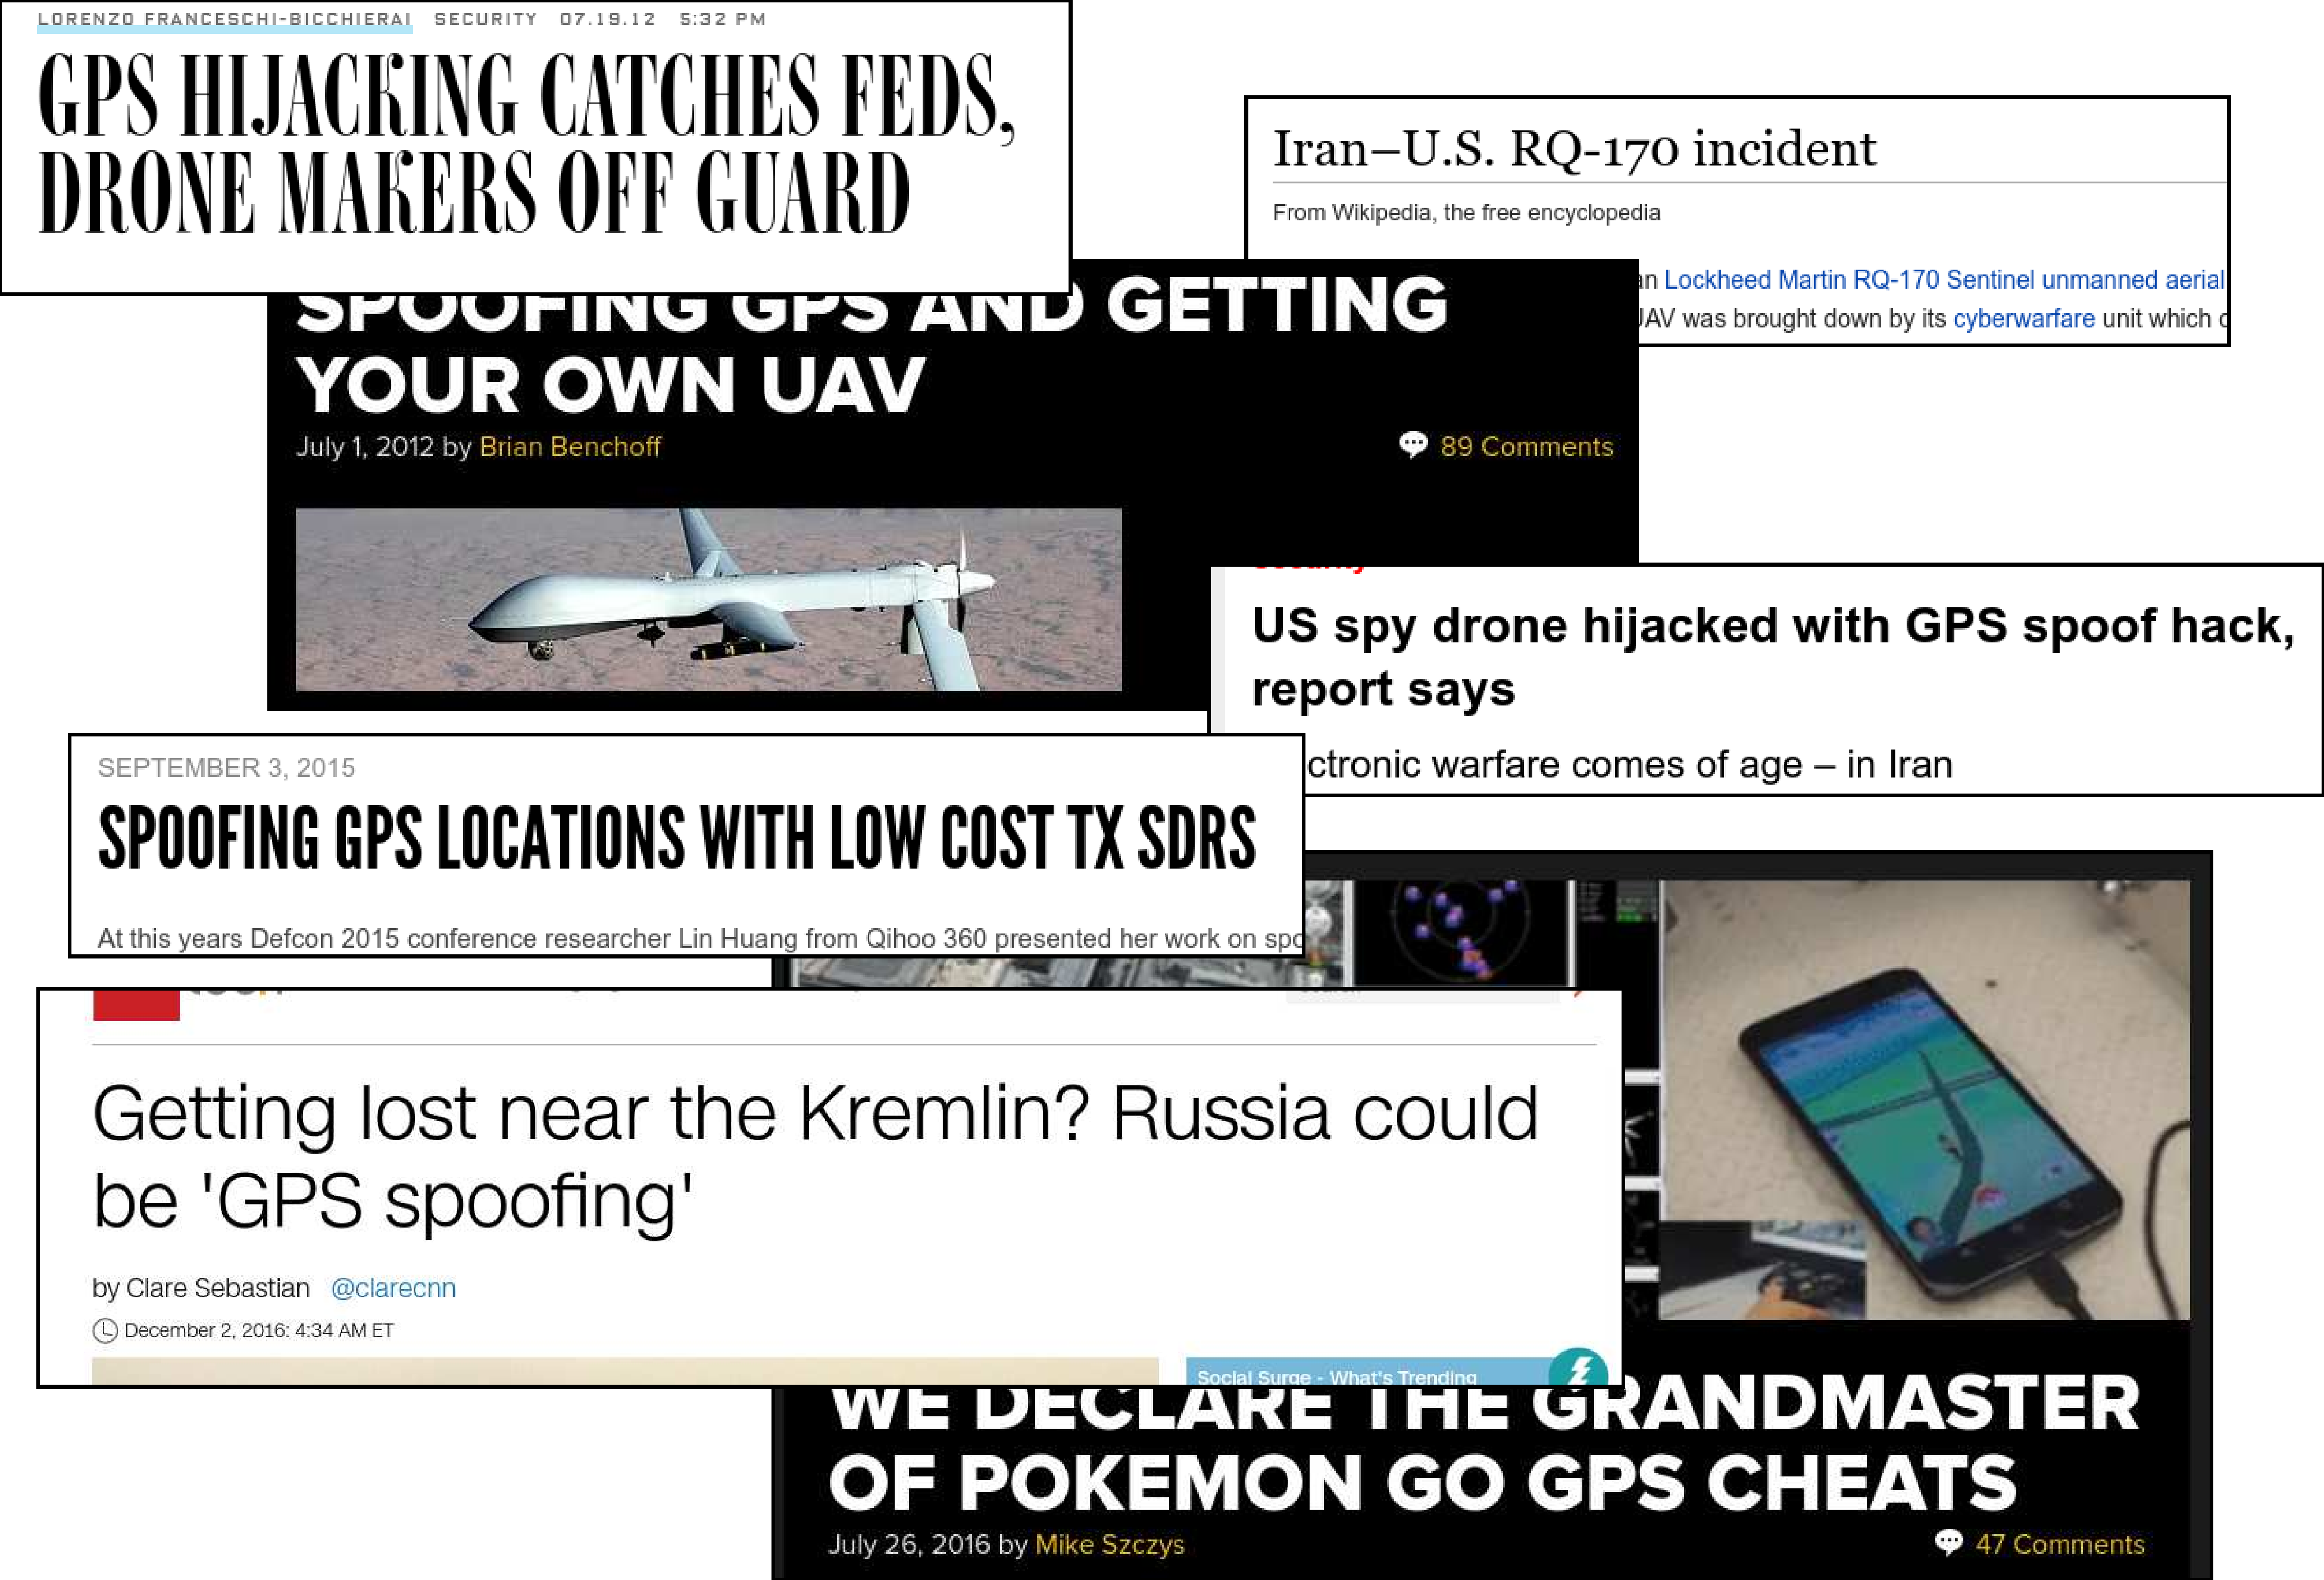
\includegraphics[scale=0.15]{thesis/graphics/montage.pdf}
      \end{figure}
%Utfordringer:
%  \begin{itemize}
%    \item Avhengig av å ha en antenne med fri sikt.
%    \item Kjent kodestruktur.
%    \item Naive mottakere.
%  \end{itemize}
%  Terror, sabotasje mulig motiv for:
%  \begin{itemize}
%    \item Jamming.
%    \item Spoofing.
%    \item Feil i utstyr.
%  \end{itemize}  
\end{frame}

\begin{frame}
\frametitle{Utfordringer og trusler}
      \begin{figure}
        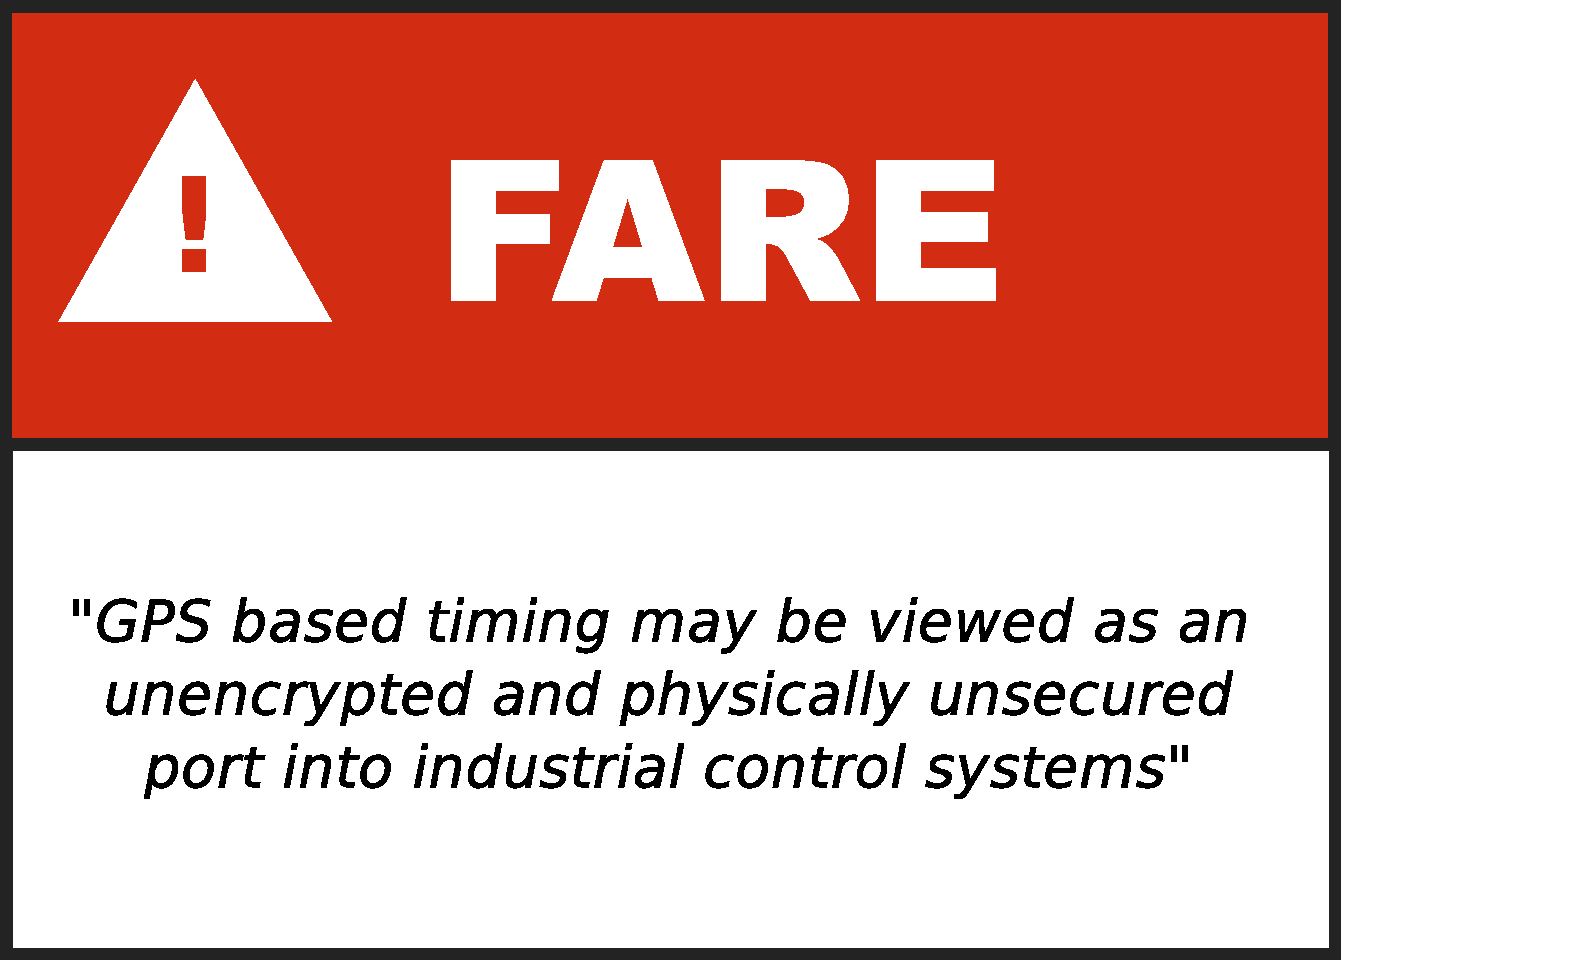
\includegraphics[scale=0.40]{thesis/graphics/fare.pdf}
      \end{figure} 
\end{frame}

\subsubsection{Referansetrusselen}
\begin{frame}
  \frametitle{"The Civil GPS Spoofer"}
  \begin{figure}
    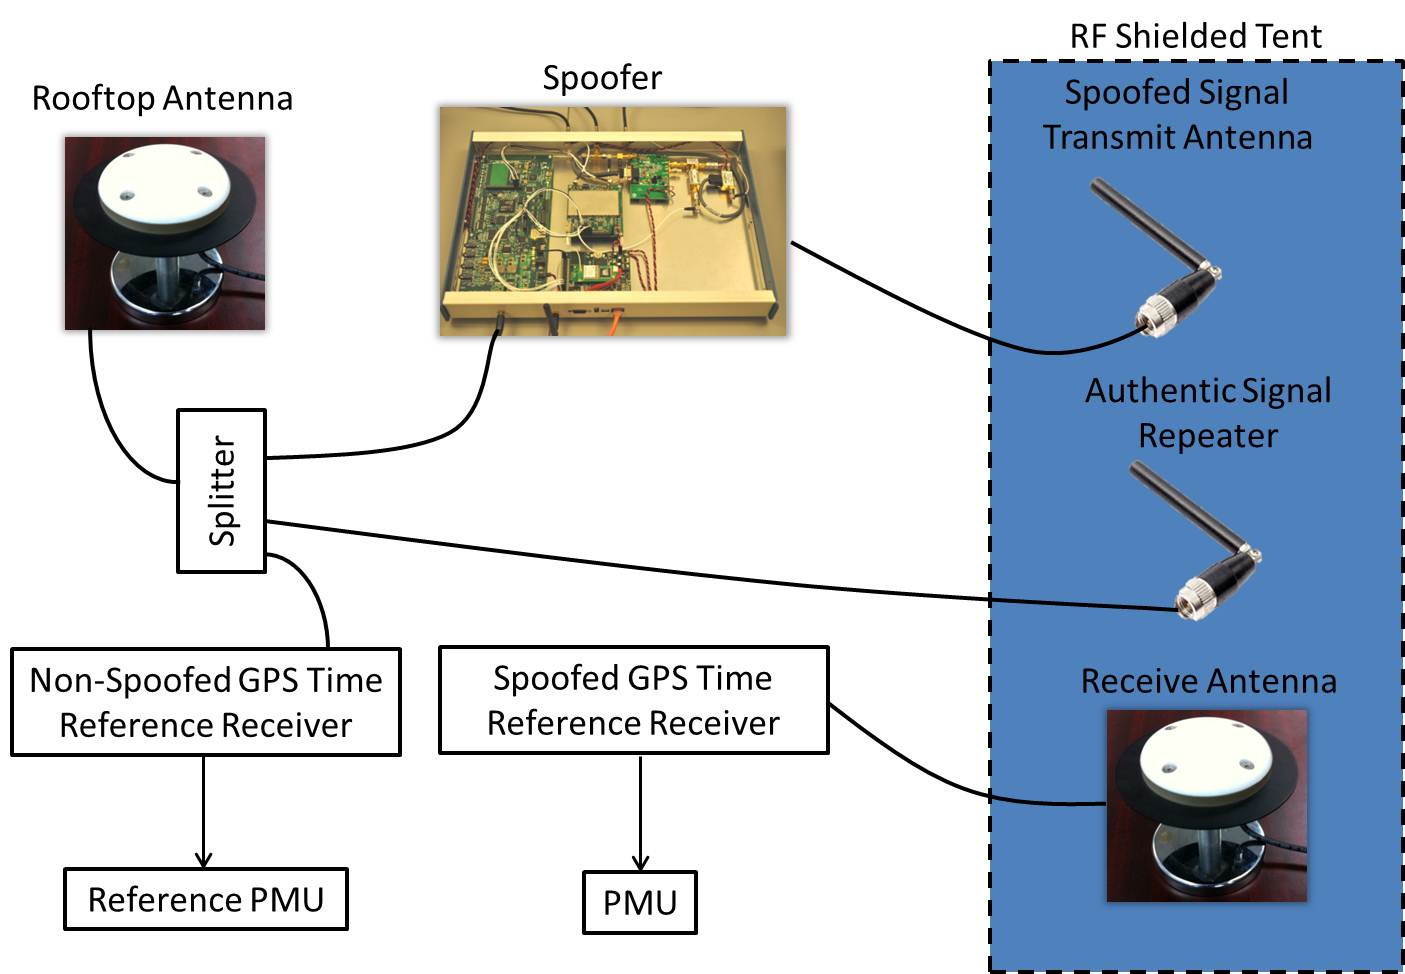
\includegraphics[scale=0.2]{thesis/graphics/spoof.jpg}
    \caption{Civil GPS Spoofer \cite{EVPMUGA}}
  \end{figure}
  %\begin{itemize}
  %  \item Laget et av et team fra \textit{The University of Texas at Austin} i 2012 \cite{EVPMUGA}
  %  \item Implementert i "SDR"
  %  \item Simulere opptil 14 "falske" satellitter.
  %\end{itemize}
\end{frame}

%\begin{frame}
%  \frametitle{"The Civil GPS Spoofer"}
%  Nøkkelfunksjoner:
%  \begin{itemize}
%    \item Sømløs narring, offeret låser på en kopi av det autentiske signalet. Ingen forandring i løsning.
%    \item Angriper manipulerer signalet.
%    \item Angriperen har gjerne et stort spillerom under angrepet da oscillatoren i mottakeren ofte er av lav kvalitet.
%  \end{itemize}
%\end{frame}

\section{Deteksjon og mottiltak}
\begin{frame}
\frametitle{Deteksjon og mottiltak}
  \begin{itemize}
      \item Bruke flere GPS mottakere med kjent posisjon og hastighet.
      \item Gode klokker -- Små korreksjoner.
    \end{itemize}
\end{frame}

\subsection{Flere GPS mottakere}
\begin{frame} 
  \frametitle{Flere GPS mottakere og kjent posisjon}
  \begin{figure}
    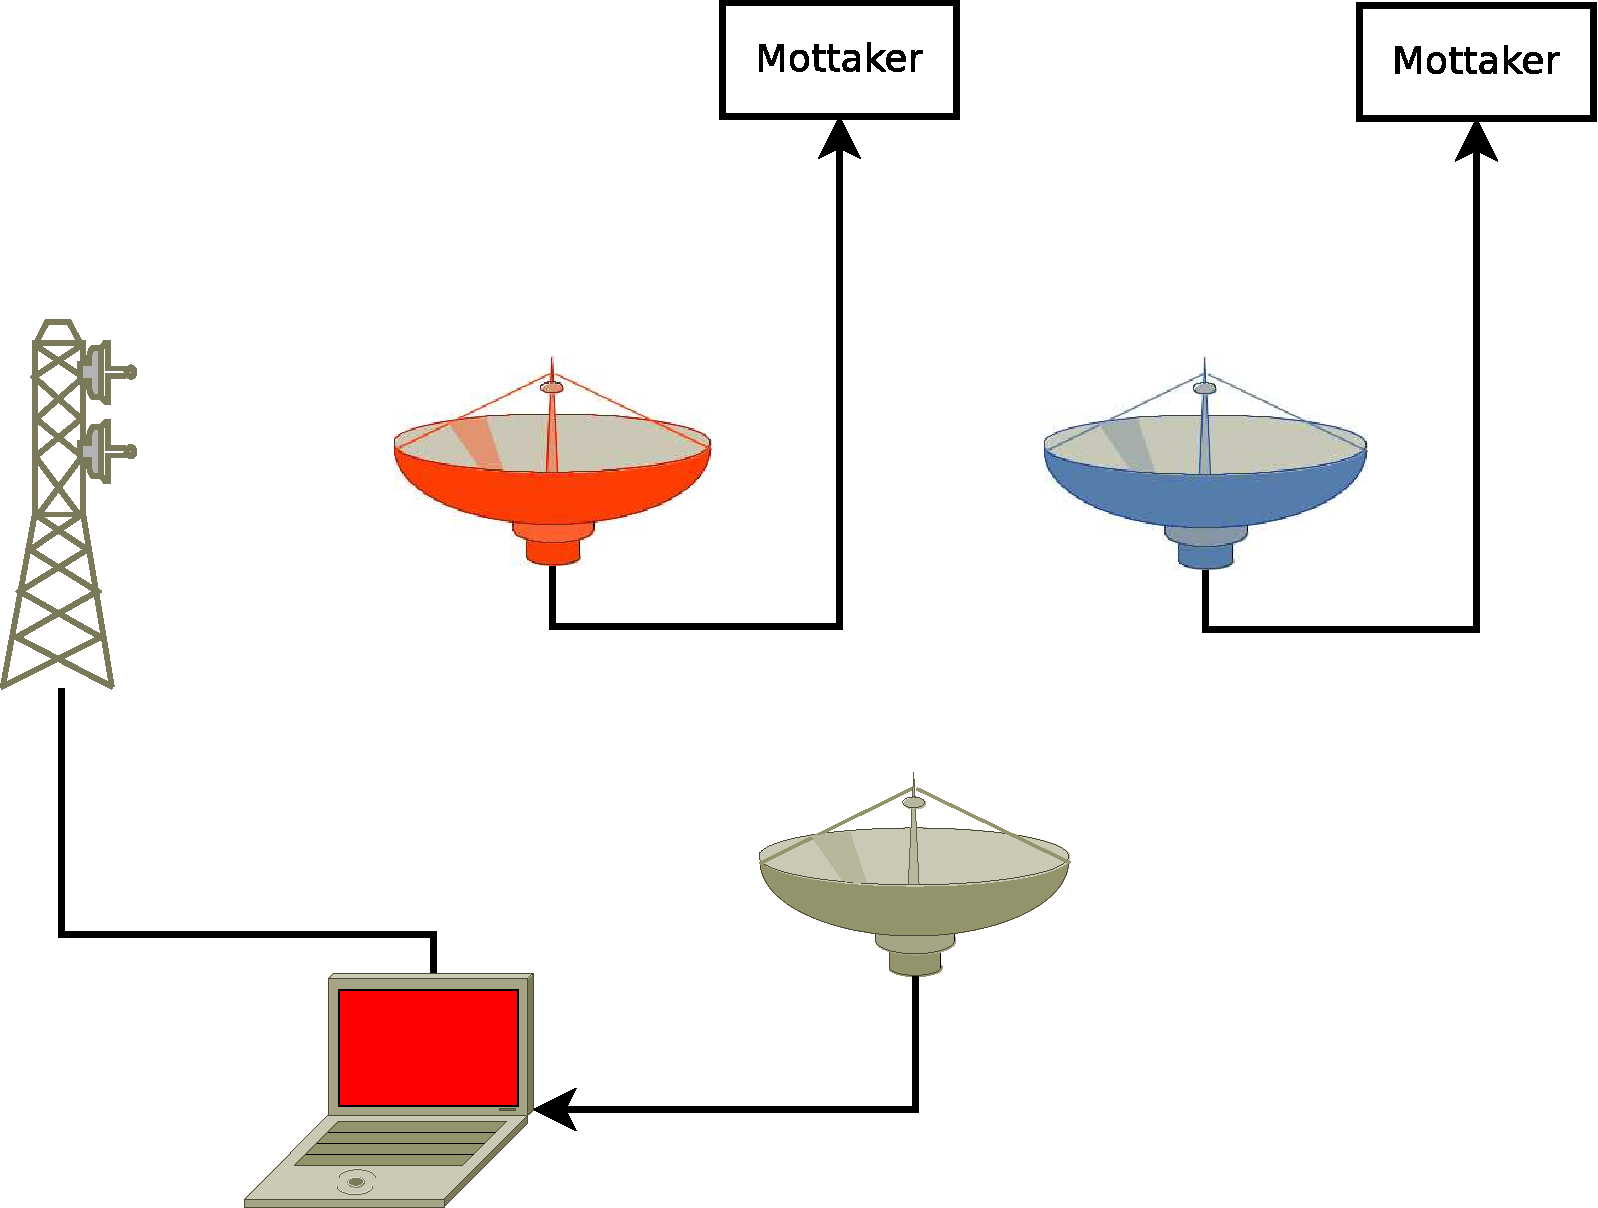
\includegraphics[scale=0.2]{thesis/graphics/toantenner.pdf}
    \caption{Spoofing deteksjon med to antenner}
  \end{figure}
\end{frame}

\begin{frame} 
  \frametitle{Flere GPS mottakere og kjent posisjon}
  \begin{figure}
    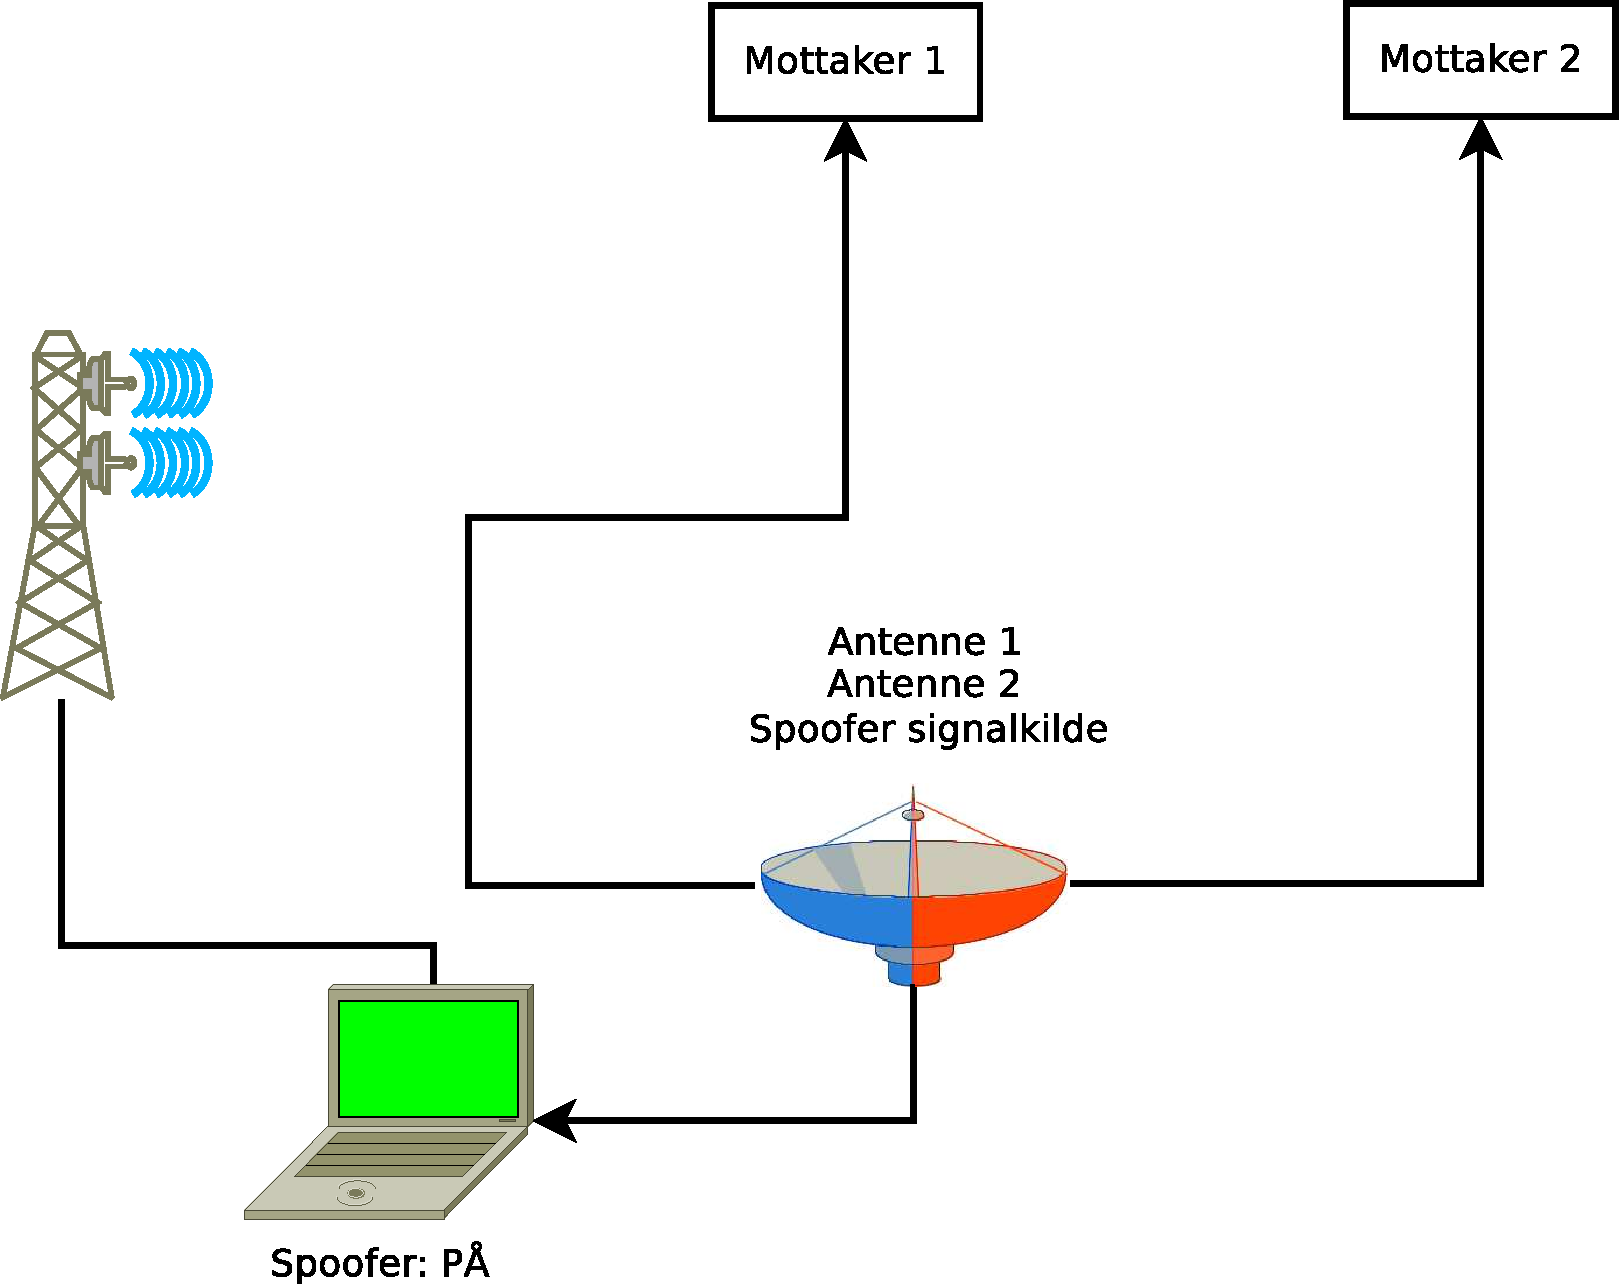
\includegraphics[scale=0.2]{thesis/graphics/toantenner_2.pdf}
    \caption{Spoofing deteksjon med to antenner}
  \end{figure}
\end{frame}

\subsection{Referanseklokke}
\begin{frame}
  \frametitle{Referanseklokke}
  \begin{columns}
    \column{0.5\textwidth}
    \begin{itemize}
      \item Trenger får korreksjoner
      \item Lite påvirket av temperatur
      \item Intern frekvensteller og styringsalgoritme
    \end{itemize}
    \column{0.5\textwidth}
      \begin{figure}
        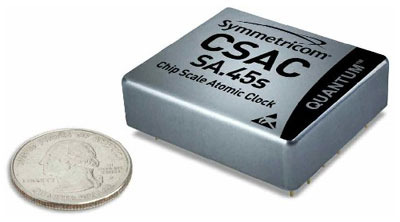
\includegraphics[scale=0.2]{thesis/graphics/csac.jpg}
      \caption{Symmetricom SA.45s CSAC}
    \end{figure}
  \end{columns}
\end{frame}

\begin{frame}
  \frametitle{Referanseklokke}
      \begin{figure}
        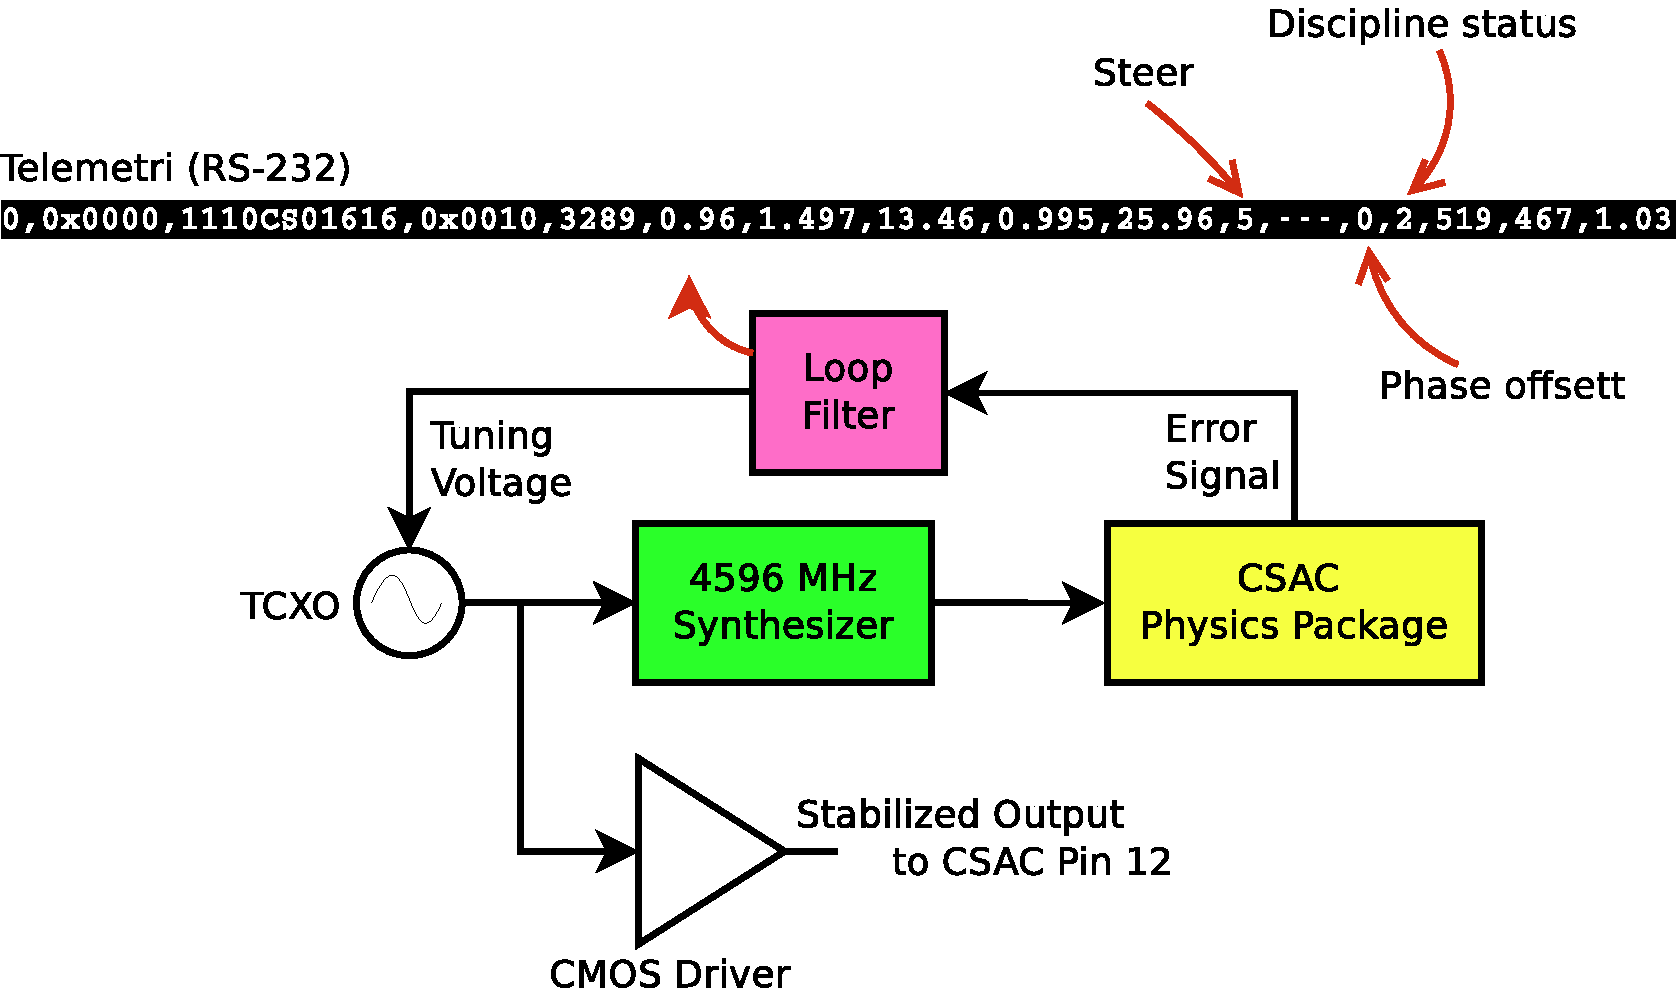
\includegraphics[scale=0.35]{thesis/graphics/csac_schematic.pdf}
      \caption{CSAC blokkdiagram}
    \end{figure}
\end{frame}

\section{Implementasjon}
\subsection{Ønsket funksjonalitet}
\begin{frame}
  \frametitle{Ønsket funksjonalitet}
  \begin{itemize}
    \item Detektere angrep:
      \begin{itemize}
        \item GPS
        \item Klokke
      \end{itemize}
    \item Logging
    \item Enkel utbygging
    \item Administreres over nettverk
    \item Konfigurerbar 
  \end{itemize}
\end{frame}

\subsection{Sensor server arkitektur}
\begin{frame}
  \frametitle{Sensor server arkitektur}
    \begin{figure}
      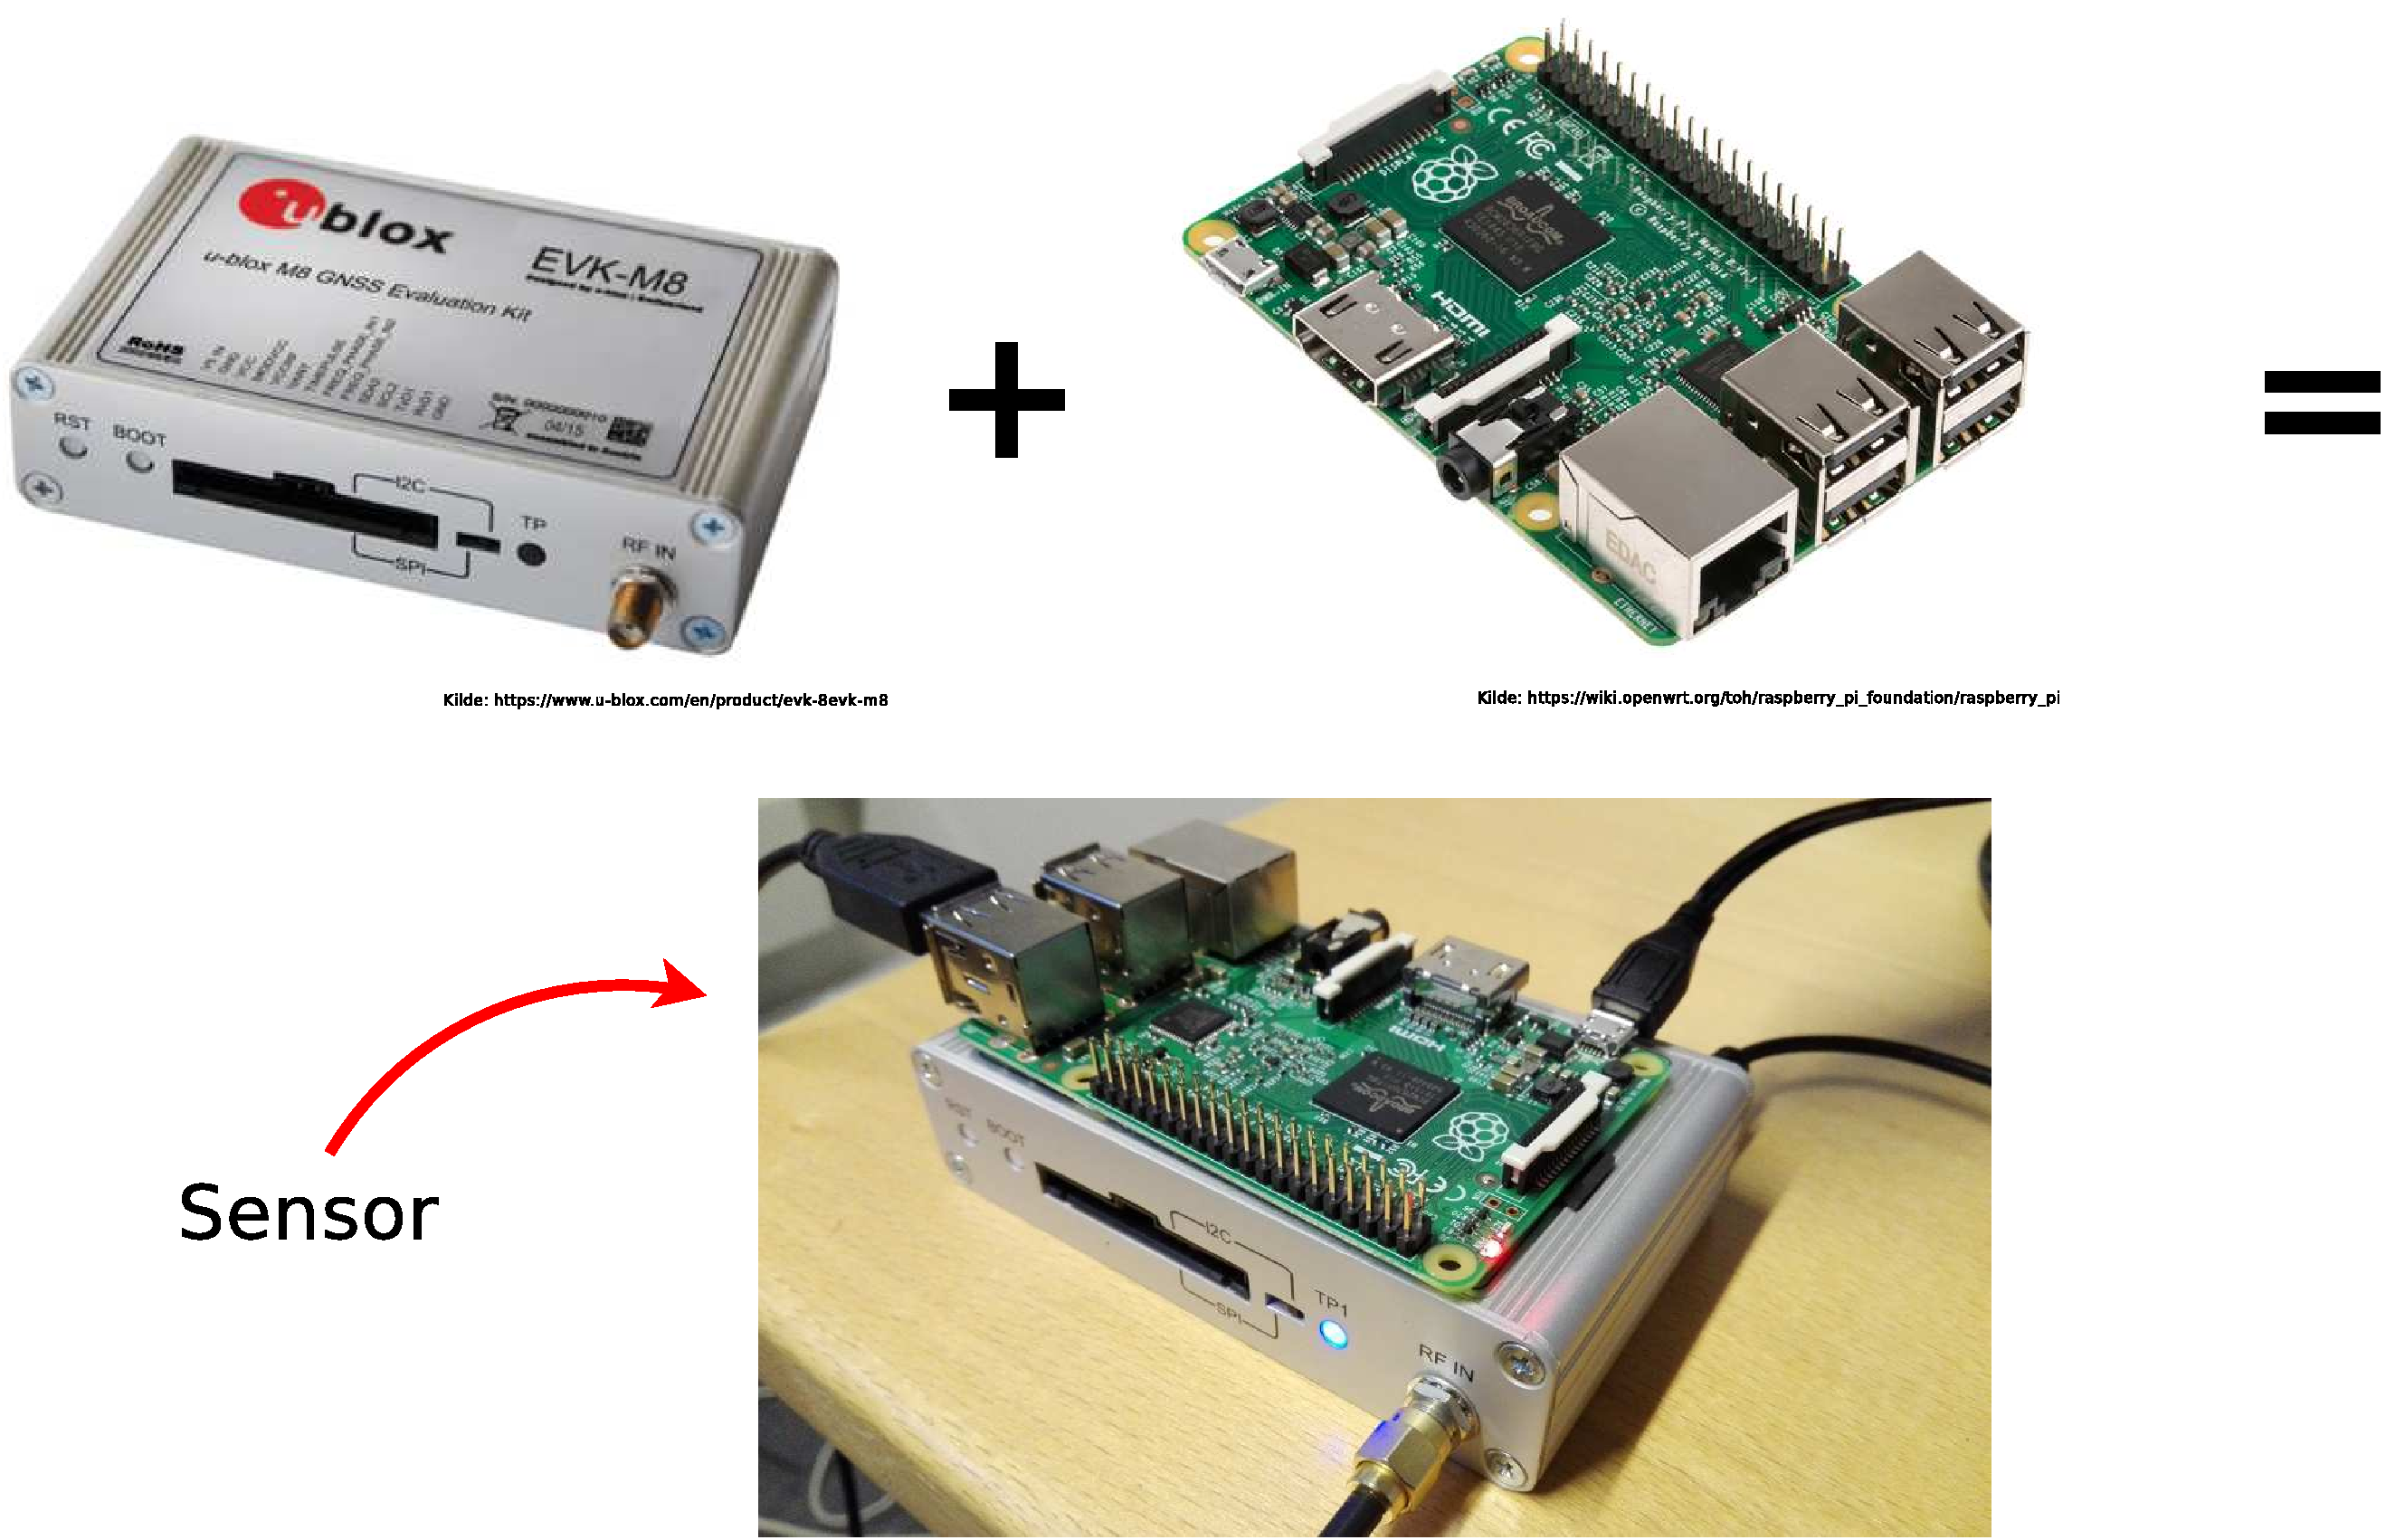
\includegraphics[scale=0.2]{thesis/graphics/raspi_gps.pdf}
    \end{figure}
  %\begin{itemize}
  %  \item Mottaker + Raspberry PI = Sensor
  %  \item Eliminerer behovet for lange signalkabler, bruke nettverk:
  %  \begin{itemize}
  %    \item Fiber
  %    \item Mobilnett (3G og 4G)
  %    \item WiFi
  %  \end{itemize}
  %  \item Antall mottakere begrenset av serverens maskinvare.
  %\end{itemize}
\end{frame}

\begin{frame}
  \frametitle{Sensor server arkitektur}
  \begin{itemize}
    \item 3000+ linjer med C99 kode
    \item Håndterer av/pålogging av klienter
    \item Håndtere mottak og formatering av GPS data
    \item En prosess per pålogging
    \item Delt minne mellom prosesser (anonym MMAP)
      \begin{itemize}
        \item Semaforer og barrierer for beskyttelse
      \end{itemize}
    \item Mulighet for brukere å koble på og gi kommandoer, f.eks:
      \begin{itemize}
        \item Rapporterer lokasjon og tid
        \item Rapportere server status
        \item Rapportere filterstatus
        \item Lagre og gjenopprette tilstand i sensorer
        \item Laste inn nye lokasjonsdata
        \item Avslutte egen og andres tilkobling
        \item Sende kommandoer til atomklokka 
      \end{itemize}
  \end{itemize}
\end{frame}

\subsubsection{Klokkemodell}
\begin{frame}
  \frametitle{Klokkemodell}
    \begin{figure}
        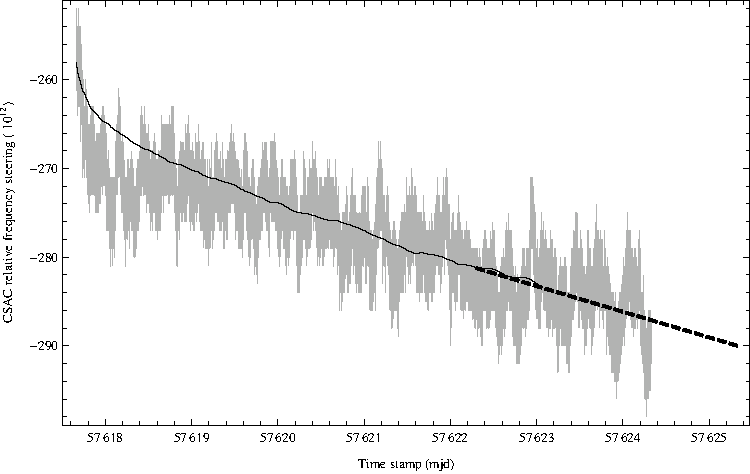
\includegraphics[scale=0.8]{thesis/graphics/csac_modelling_prediction.pdf}
      \caption{CSAC styringskorreksjon, fra klokke og predikert.}
    \end{figure}
    %Klokkemodellen brukt i oppgaven er designet av Harald Hauglin. Brukes til:
    %\begin{itemize}
    %  \item Referanse for frekvensavvik og klokkedrift 
    %  \item Generere brukbare styringsparameter i tilfelle GPS løsning ikke lenger er til å stole på.
    %\end{itemize}
    %Modellen er logisk en del av serveren og kjører i en egen prosess.
    %\begin{itemize}
    %  \item Kommuniserer med atomklokka
    %  \item Moden etter to dager (konfigurerbart).
    %\end{itemize}
\end{frame}

\subsubsection{Filtre}
\begin{frame}
  \frametitle{Filtre}
  Filtrene brukes til å detektere avvik. Enten:
        \begin{itemize}
          \item GPS-basert
          \item Klokkemodell-basert
        \end{itemize}
  For øyeblikket kun implementert tre filtre:
  \begin{itemize}
    \item Lokasjon og hastighetsfilter
                  \begin{itemize}
                    \item Data fra sensorene blir samlet formatert.
                    \item Sjekker løst posisjon og hastighet mot referanseverdier
                  \end{itemize}
    \item Fasehoppfilter
                    \begin{itemize}
                      \item Sammenlikner nåværende fase med pre-konfigurert grense.
                    \end{itemize}
    \item Frekvenskorreksjonsfilter
                    \begin{itemize}
                      \item Sammenlikner nåværende styringsverdi med en forventet styringsverdi
                    \end{itemize}
  \end{itemize}
  Pre-konfigurerte referanseverdier er basert på et gjennomsnitt kalkulert fra en lengre måleserie.
\end{frame}

\section{Test av lokasjon- og hastighetsfilter}
\begin{frame}
\frametitle{Oppsett}
  \subsection{Beskrivelse}
      \begin{figure}
        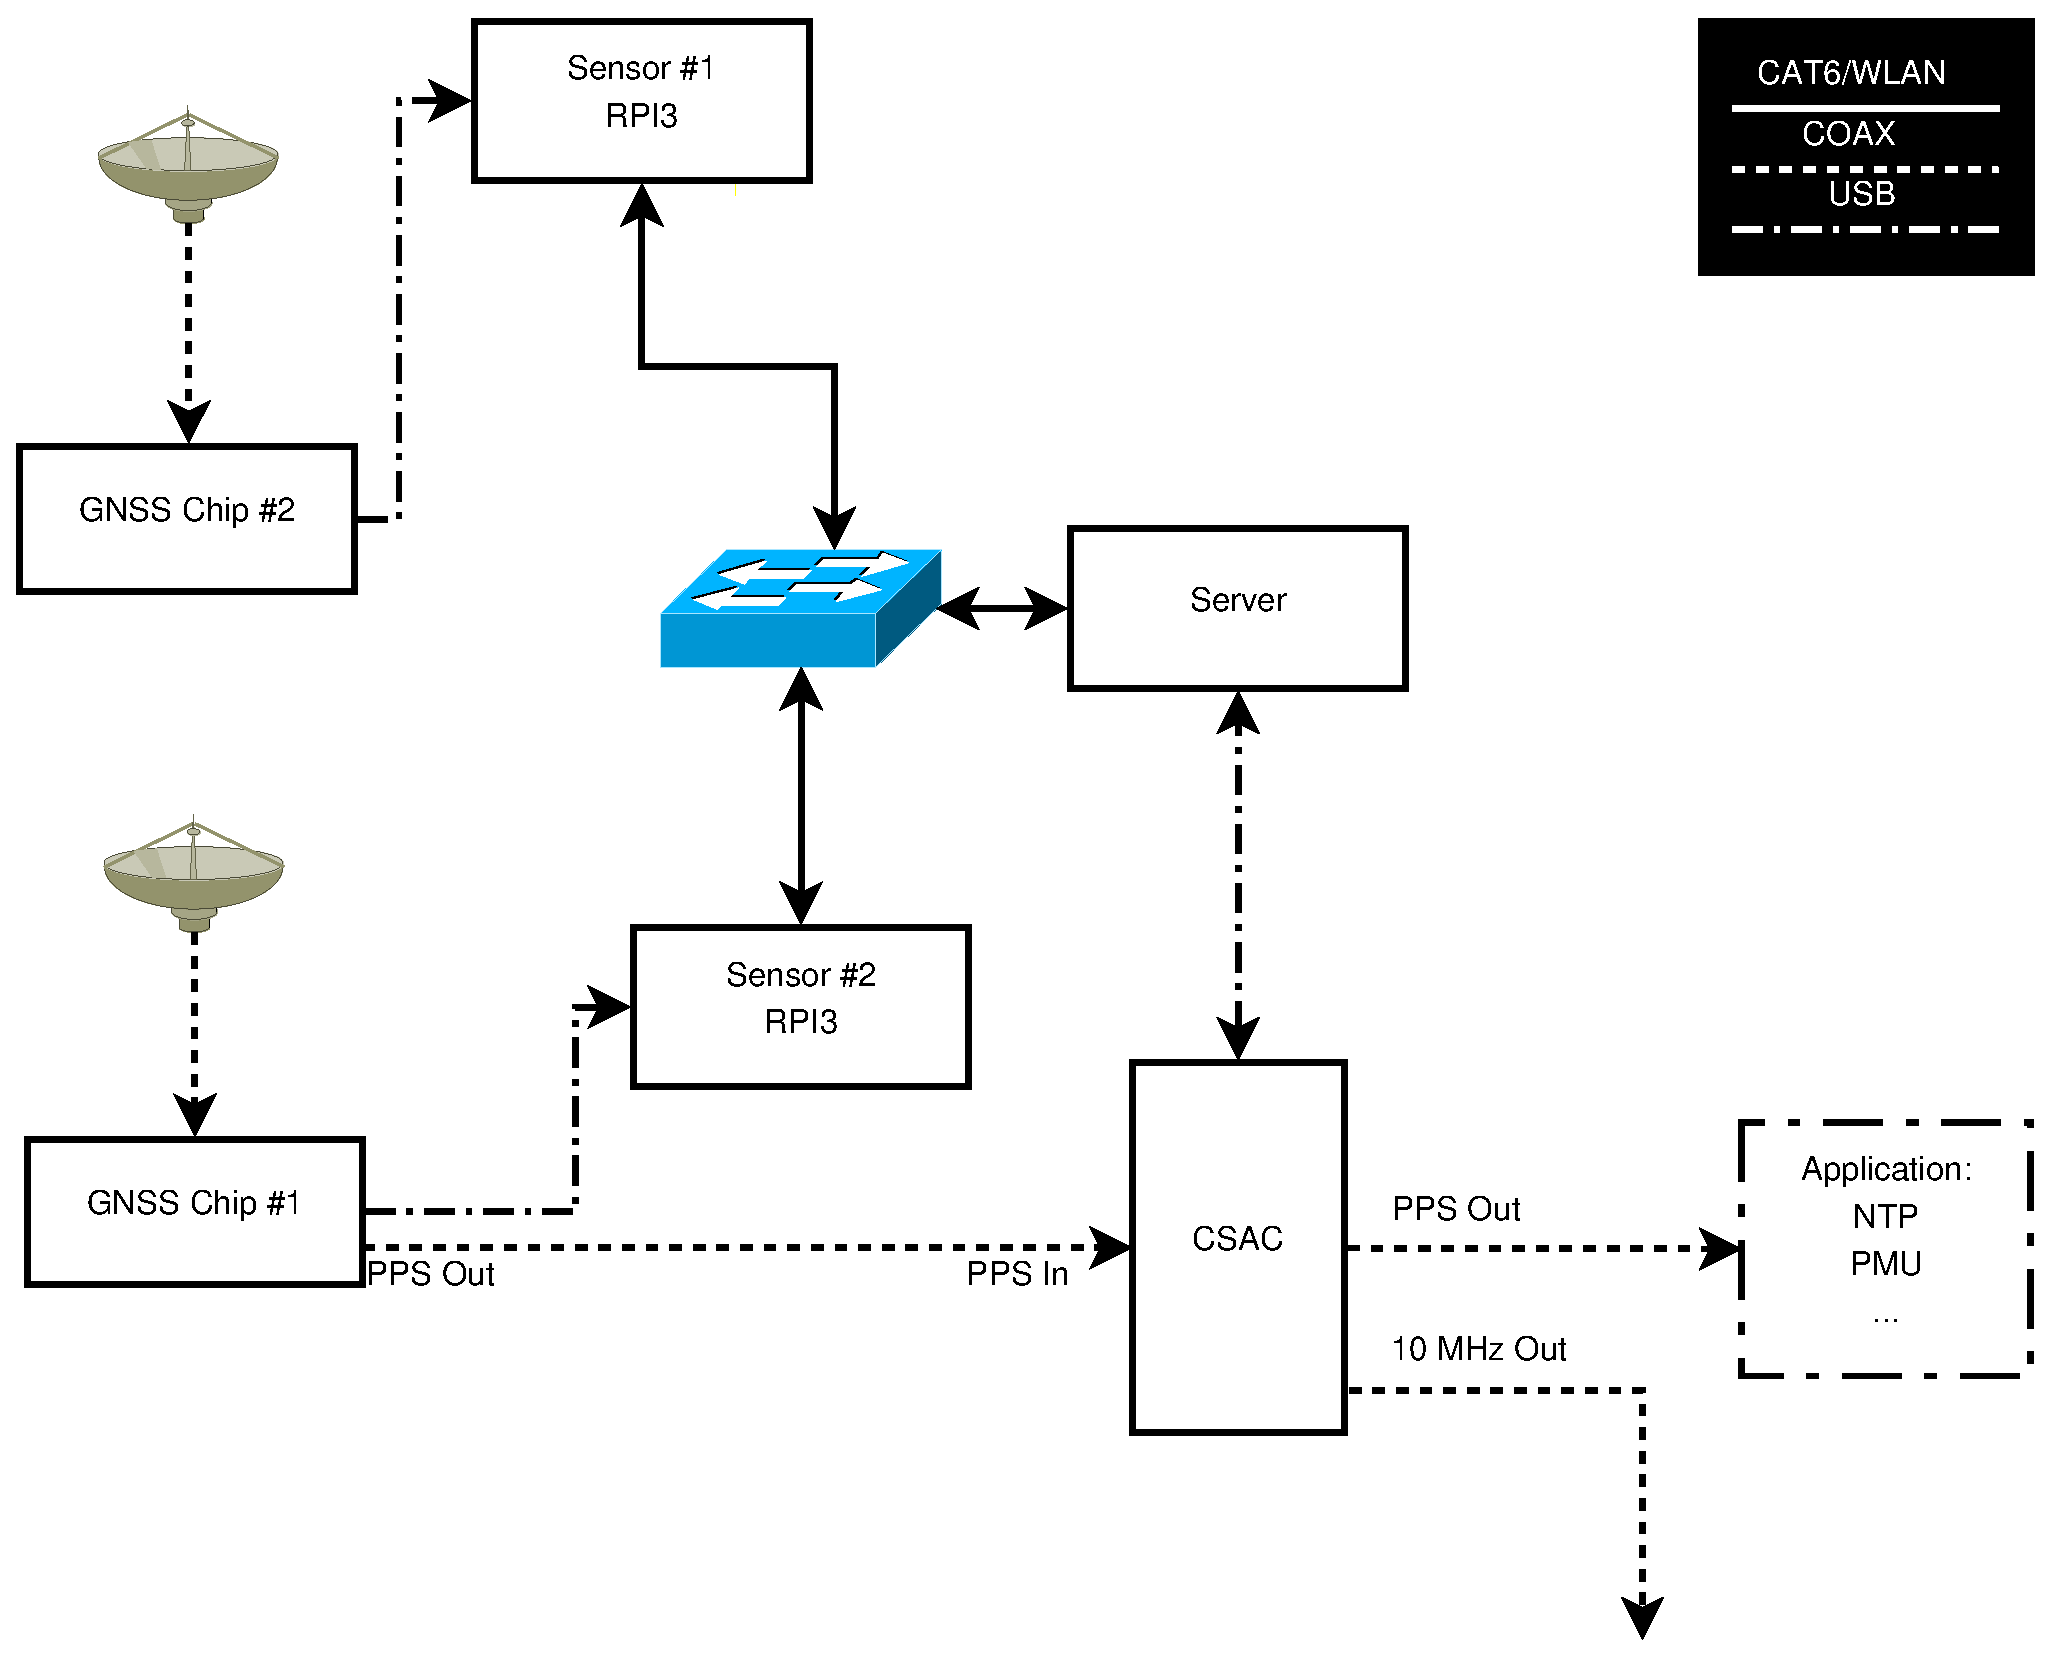
\includegraphics[scale=0.25]{thesis/graphics/server_layout.eps}
        \caption{Oppsett av server og klienter under test}
      \end{figure}
\end{frame}

\begin{frame}
\frametitle{Oppsett}
      \begin{figure}
        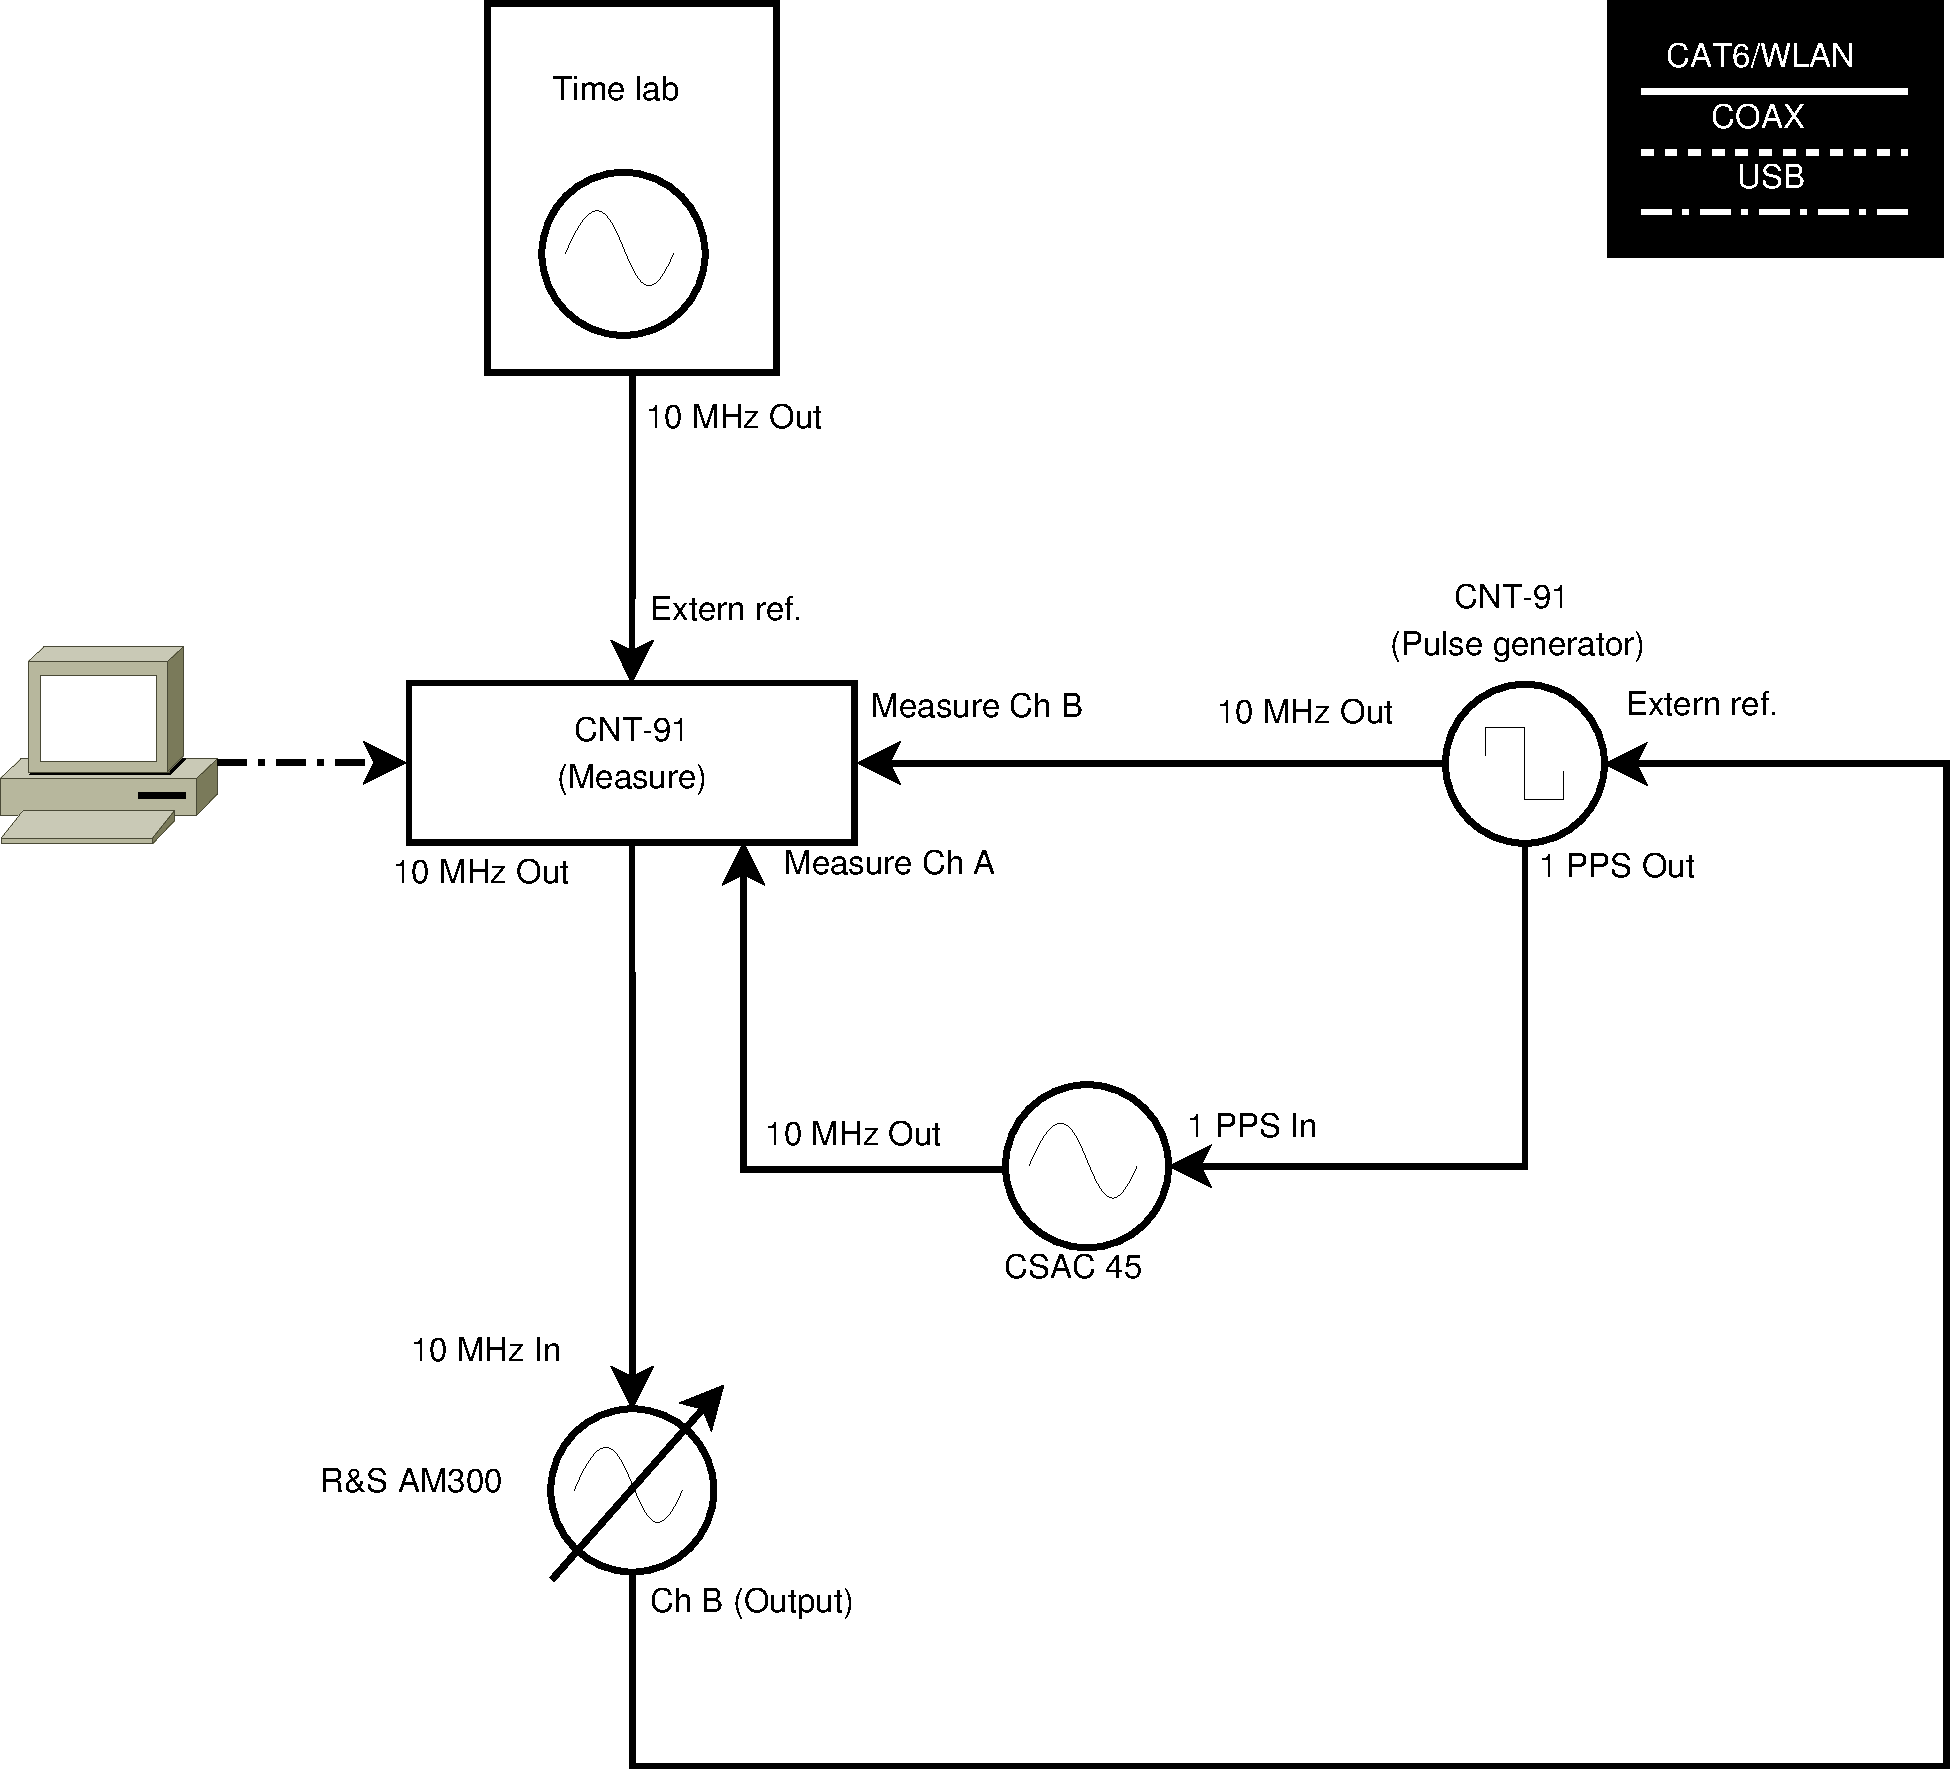
\includegraphics[scale=0.25]{thesis/graphics/measure_setup.pdf}
        \caption{Oppsett av måleutstyr}
      \end{figure}
\end{frame}

\begin{frame}
\frametitle{Oppsett: plassering av mottakere}
      \begin{figure}
        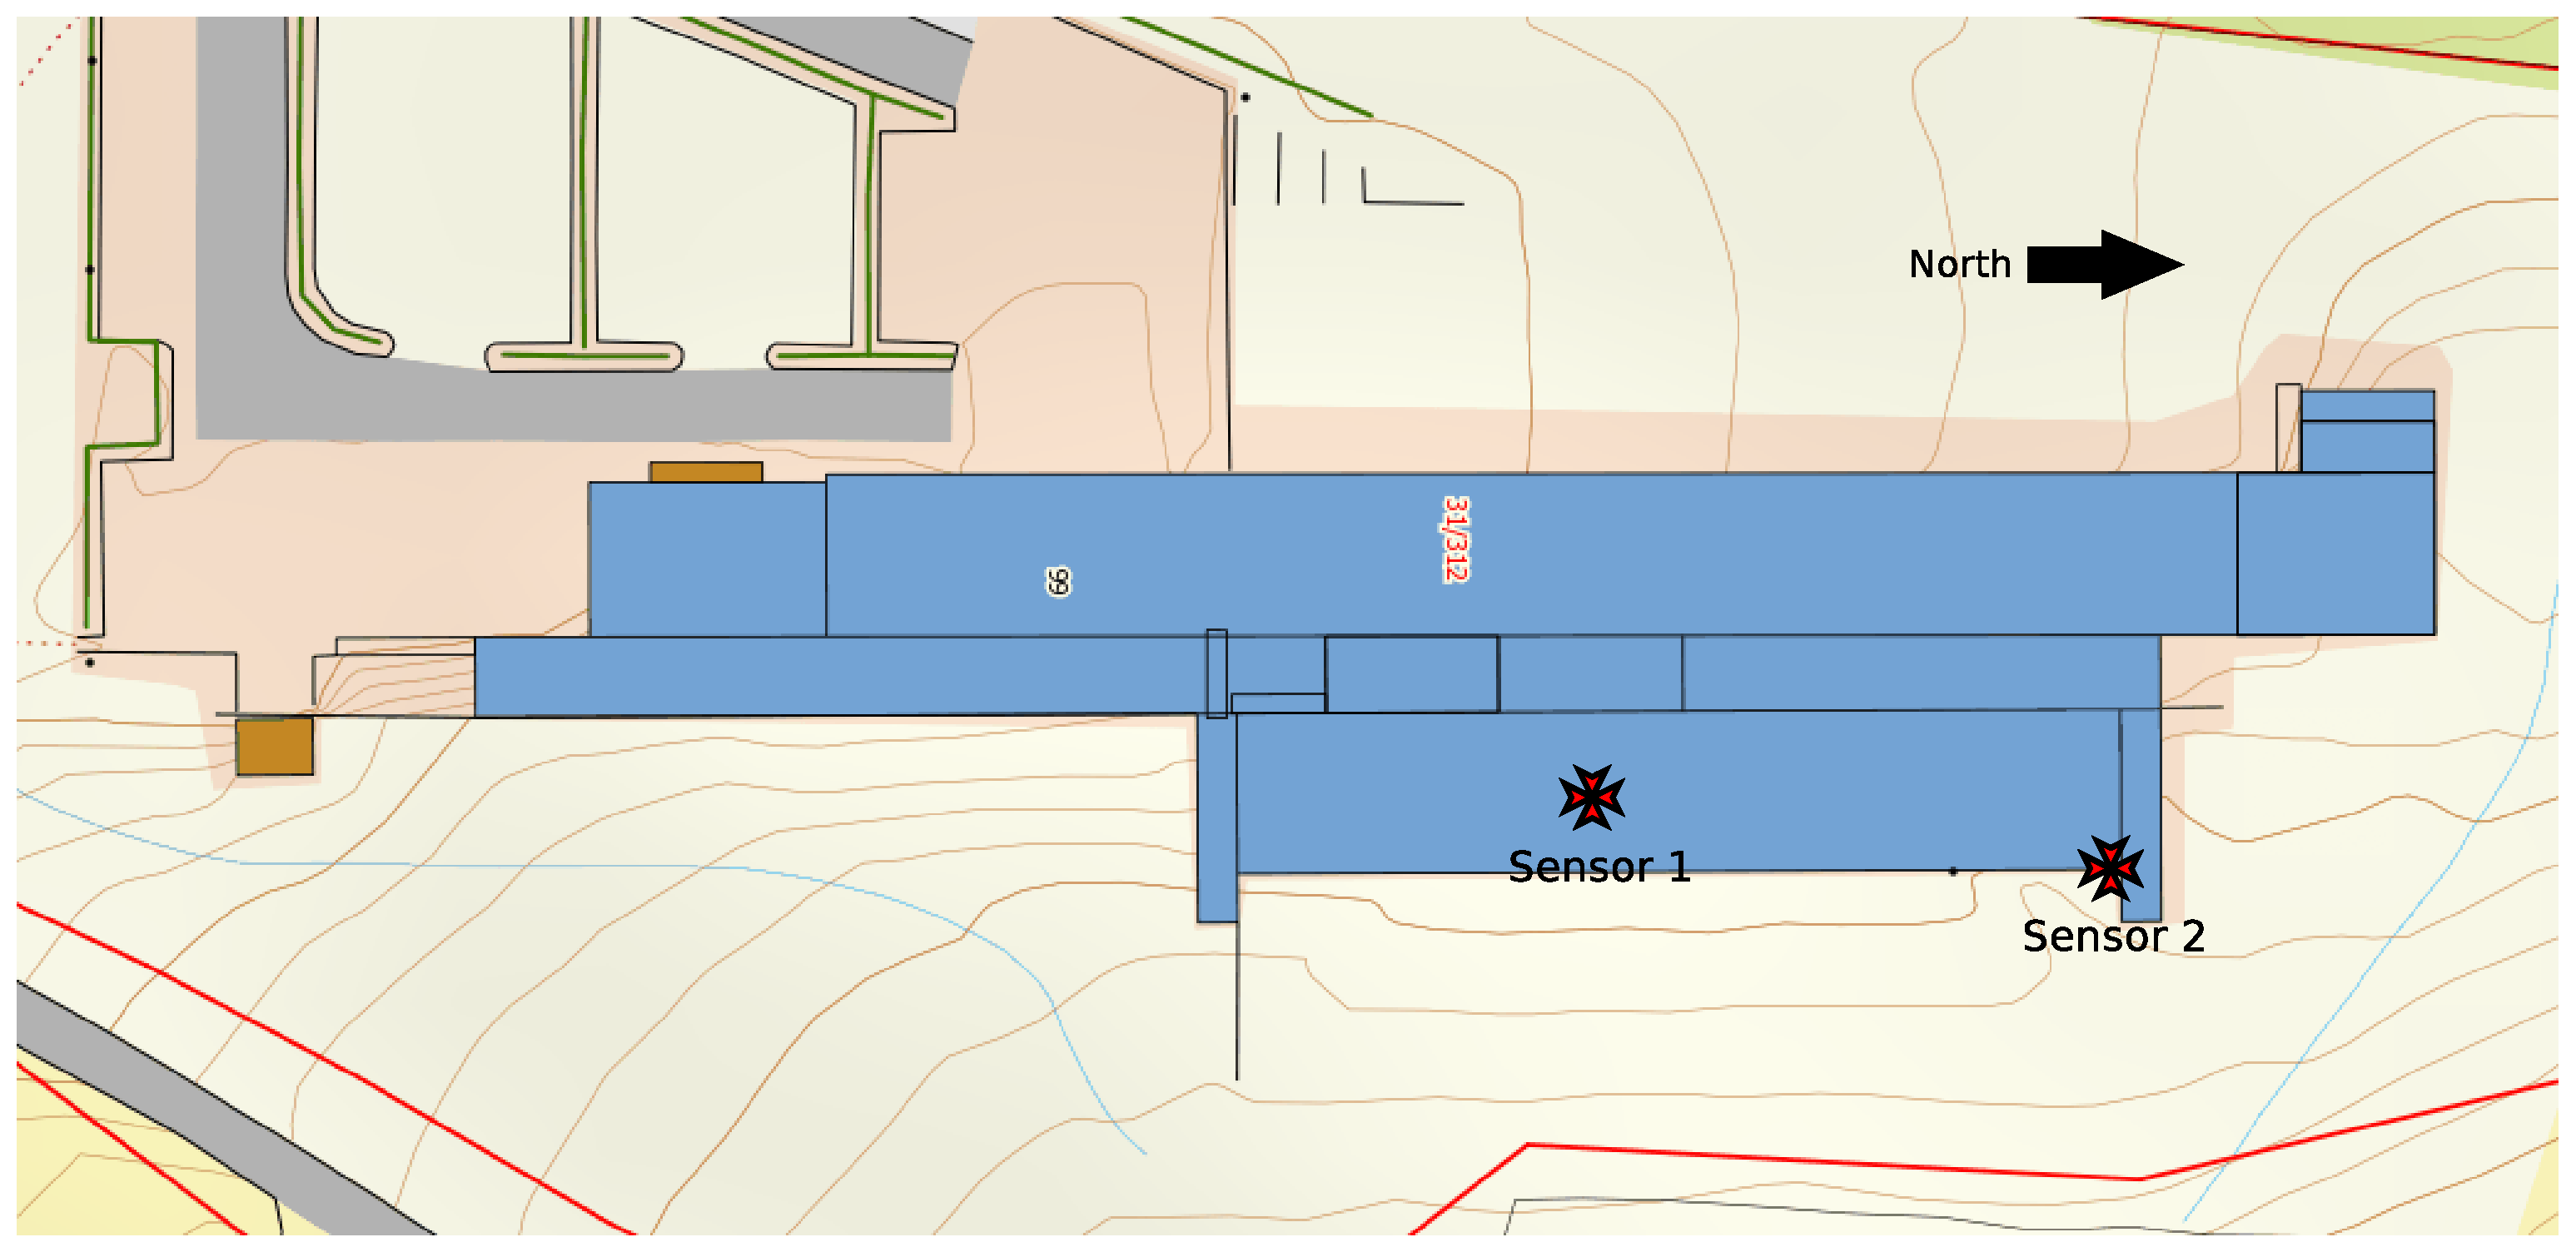
\includegraphics[scale=0.18]{thesis/graphics/roof.eps}
        \caption{Plasseringen av GPS mottakere}
      \end{figure}
\end{frame}

\begin{frame}
\frametitle{Utførelse}
      \begin{itemize}
        \item Flyttet antenne 1 mot antenne 2
        \item Flyttet antenne 2 mot antenne 1
        \item Viftet antenne 1 rundt i en halvsirkel
        \item Viftet antenne 2 rundt i en halvsirkel
        \item Dekket antennene
      \end{itemize}
\end{frame}

\begin{frame}
\frametitle{Utførelse}
\begin{center}
\begin{tikzpicture}
  \node (img1) {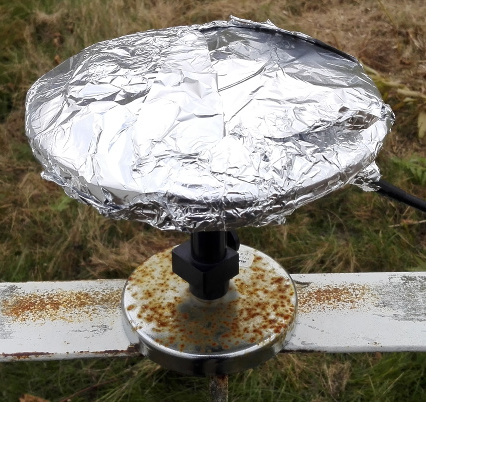
\includegraphics[height=5cm]{thesis/graphics/antenna_foil_over_hacked.jpg}};
  \node (img2) at (img1.south east) {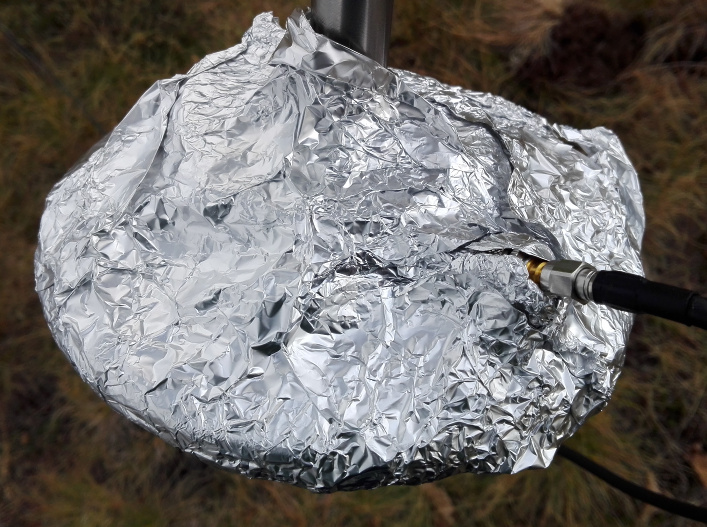
\includegraphics[height=4.5cm]{thesis/graphics/antenna_foil_cover.jpg}};
\end{tikzpicture}
\end{center}
\end{frame}

\begin{frame}
\frametitle{Observasjon}
      \begin{itemize}
        \item Ingen falske positive
        \item GPS log korrelerer
        \item Server log korrelerer
        \item Frekvensmåling korrelerer
      \end{itemize}
\end{frame}

\begin{frame}
\frametitle{Observasjon: Målesystem}
      \begin{figure}
        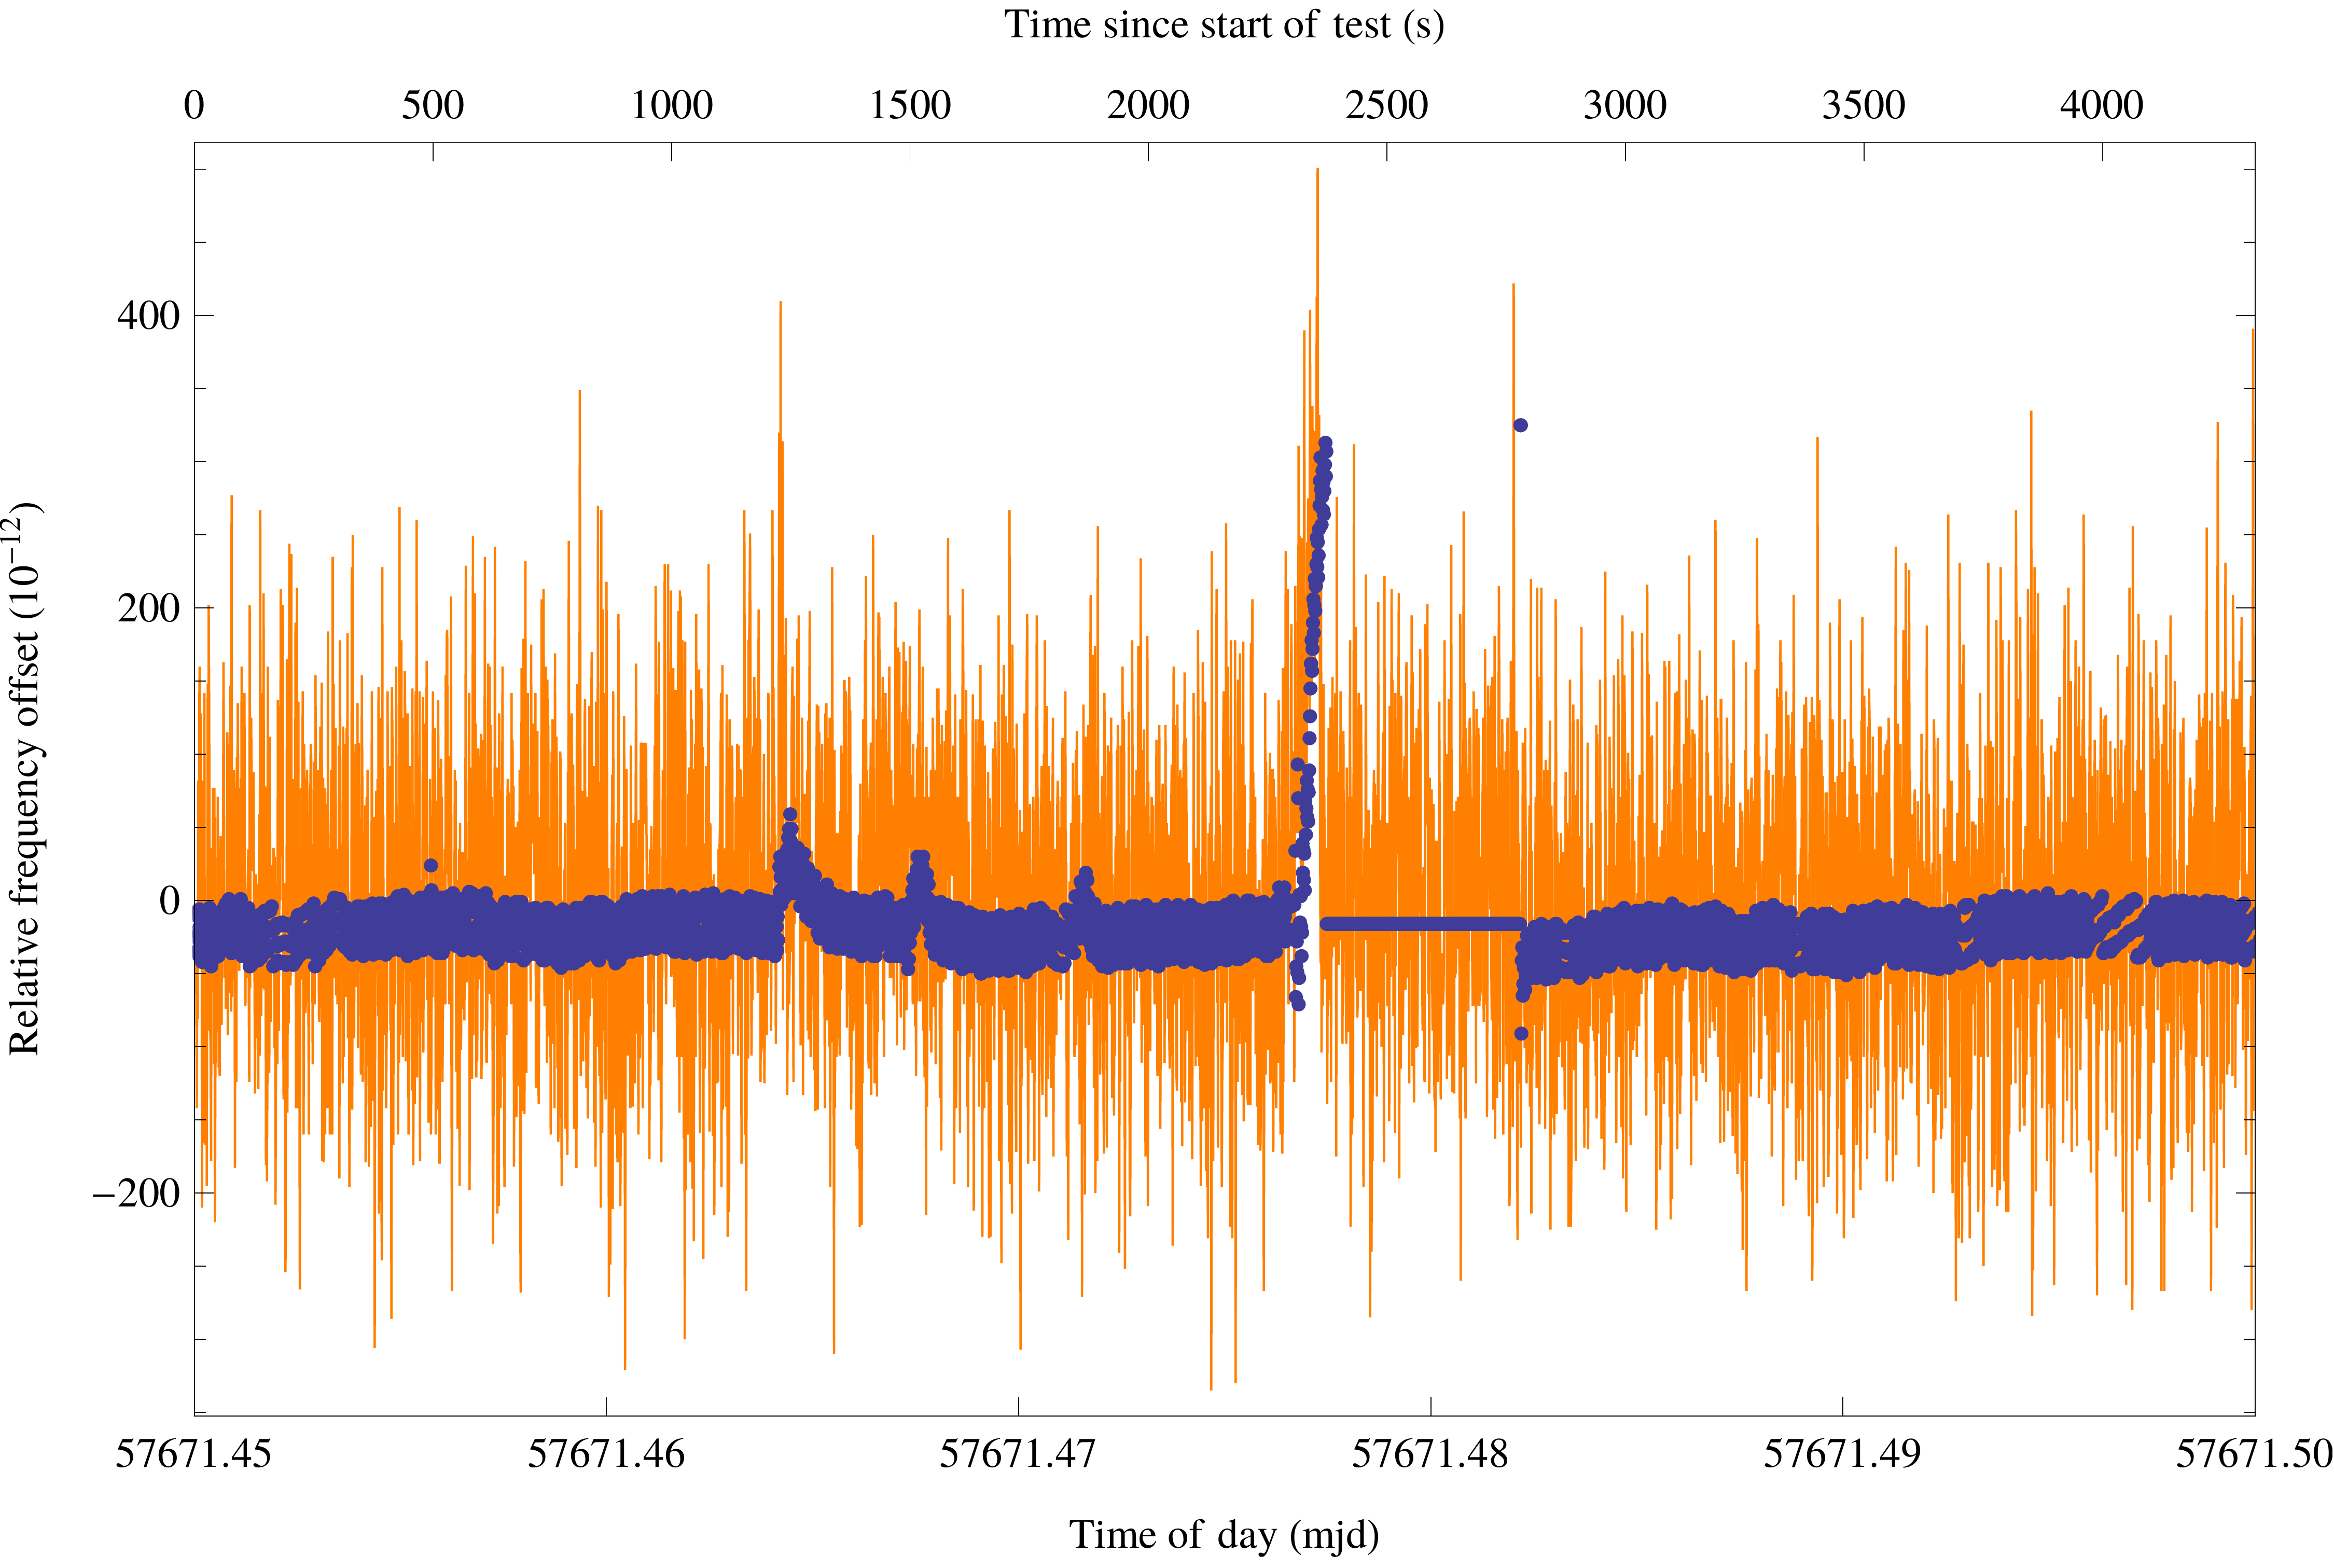
\includegraphics[scale=0.70]{thesis/graphics/cns91-and-csac-telemetry-frequency-1.png}
        \caption{Måleserie gjort under test av lokasjon og hastighetsfilter}
      \end{figure}
\end{frame}

\section{Test av klokkemodell og filtre}
\begin{frame}
\frametitle{Oppsett}
  \begin{itemize}
    \item Testet klokkemodellen og styring.
    \item Tok bare med en sensor da fokus var på klokkemodell.
    \item Justerte grenseverdier
  \end{itemize}
\end{frame}

\begin{frame}
\frametitle{Utførelse}
      \begin{itemize}
        \item Flyttet antenne 
        \item Viftet antenne rundt i en halvsirkel
        \item Aktiverte disiplinering av klokka manuelt
      \end{itemize}
\end{frame}

\begin{frame}
\frametitle{Observasjon}
      \begin{itemize}
        \item Ingen falske positive
        \item GPS log korrelerer
        \item Server log korrelerer
        \item Frekvensmåling korrelerer
      \end{itemize}
\end{frame}

\begin{frame}
\subsection{Observasjon}
\frametitle{Observasjon}
      \begin{figure}
        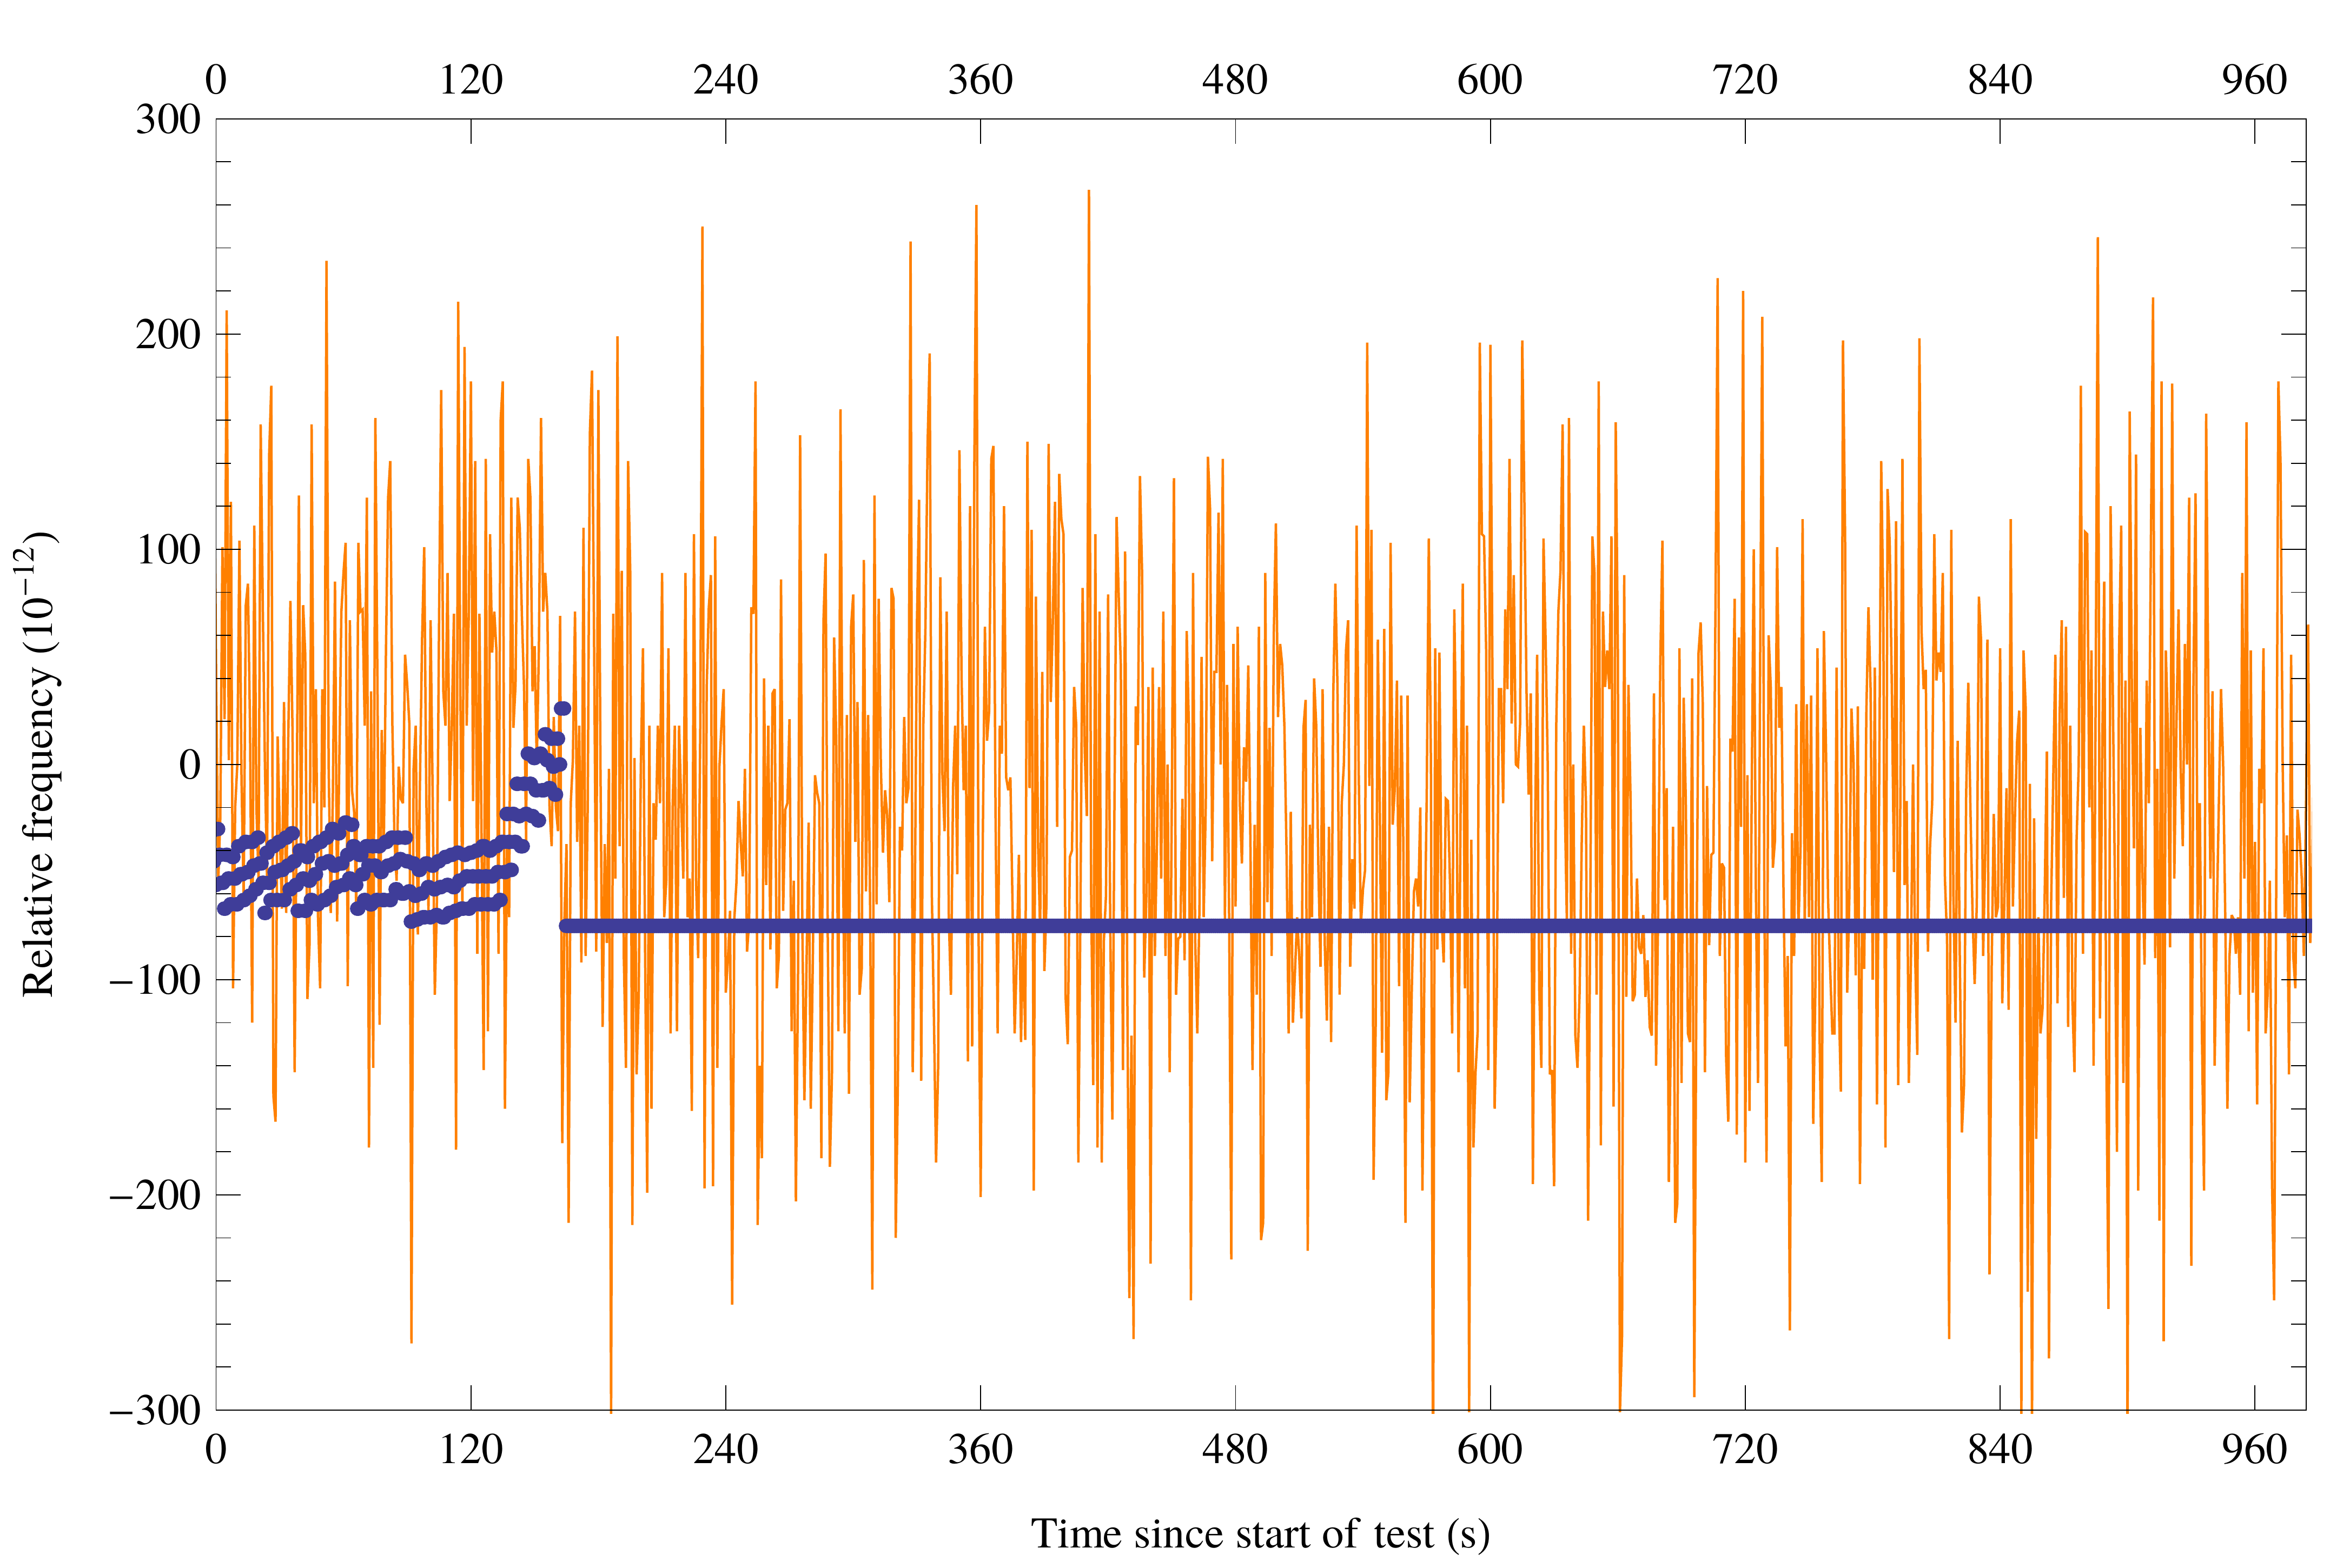
\includegraphics[scale=0.70]{thesis/graphics/20161024-test2-telemetry-and-cnt91-combined-1-2.png}
        \caption{Måleserie gjort under klokkemodell test}
      \end{figure}
\end{frame}

\section{Konklusjon}
\begin{frame}
  \frametitle{Konklusjon}
  Vi har demonstrert:
  \begin{itemize}
    \item At en fullt fungerende \textit{"spoof proof atomic clock controller"} ville ha vært i stand til å stå imot et angrep utført med en sofistikert GPS spoofer slik som \textit{"The Civil GPS spoofer"}.
    \item Nåværende implementasjonen evne til å detektere en forstyrrelse av GPS signaler og en begrenset evne til å begrense skaden av nevnte forstyrrelse.
    \item Effektivitet til Sensor server arkitekturen. 
    \begin{itemize}
      \item Lav responstid
      \item Høy stabilitet 
      \item Enkel å bygge ut med flere sensorer
    \end{itemize}
  \end{itemize}
\end{frame}

\section{Etter innlevering}
\begin{frame}
  \begin{itemize}
  \item Kommunikasjon med atomklokke
    \frametitle{Ikke løste problemer}
    \begin{itemize}
      \item Antatt å ha vært et problem med konfigurasjonen av serialport.
      \item Systematisk feilsøkt etter innlevering. Forsøkt:
      \begin{itemize}
        \item Forskjellige kabler
        \item Forskjellige datamaskiner
        \item Verifisert med "serial port sniffer", riktig kommando sendes.
      \end{itemize}
      \item Kan være et fastvare problem
    \end{itemize}
  \item GPS filter ikke ferdig integrert.
  \end{itemize}
\end{frame}

\section{Bibliografi}
\begin{frame}[allowframebreaks]%in case more than 1 slide needed
  \frametitle{Bibliografi}
  \printbibliography[heading=bibintoc]
\end{frame}

\end{document}